\documentclass[11pt]{scrartcl}
\usepackage{graphicx}
\usepackage{tikz}
\usetikzlibrary{angles,quotes}
\usetikzlibrary{patterns}
\usetikzlibrary{calc}
\usepackage{tkz-euclide}
\graphicspath{{./}}
\usepackage[sexy,fancy]{evan}
\usepackage[normalem]{ulem}
\usepackage{hyperref}
\usepackage{mathtools}
\hypersetup{
    colorlinks=true,
    linkcolor=blue,
    filecolor=magenta,      
    urlcolor=cyan,
    pdftitle={Educational PDF by Azzam},
    pdfpagemode=FullScreen,
    }

\usepackage{listings}
\usepackage{xcolor}
\lstset { %
    language=C++,
    backgroundcolor=\color{black!5}, % set backgroundcolor
    %basicstyle=\footnotesize,% basic font setting
}
 
\renewcommand{\baselinestretch}{1.5}

\addtolength{\oddsidemargin}{-0.4in}
\addtolength{\evensidemargin}{-0.4in}
\addtolength{\textwidth}{0.8in}
% \addtolength{\topmargin}{-0.2in}
% \addtolength{\textheight}{1in} 

\setlength{\parindent}{0pt}

\usepackage{pgfplots}
\pgfplotsset{compat=1.15}
\usepackage{mathrsfs}
\usetikzlibrary{arrows}

\begin{document}
\title{Basic Lessons on High School Math Olympiad}
\date{\today}
\author{Azzam L. H. (Instagram: azzam\_29\_12)}
\maketitle
\renewcommand*\contentsname{Daftar Isi}
\tableofcontents
\newpage
\section{Aljabar}
\subsection{Pemfaktoran dan Penguraian}
Tips: Jangan dihafal secara sengaja, tetapi banyak-banyaklah latihan soal, nanti hafal sendiri :D.
	
	Untuk $x,y,z \in \CC$.

        \subsubsection{\textit{Basic} yang paling sering muncul}
        \begin{enumerate}
            \item $x^2-y^2 = (x+y)(x-y)$.
	    \item $(x+y)^2 = x^2+2xy+y^2$.
	    \item $(x-y)^2 = x^2-2xy+y^2$.
            \item $(x+y)^3 = x^3+y^3+3xy(x+y) = x^3+3x^2y+3xy^2+y^3$. 
	    \item $(x-y)^3 = x^3-y^3+3xy(x-y) = x^3-3x^2y+3xy^2-y^3$. 
	    \item $x^3-y^3 = (x-y)(x^2+xy+y^2)$.
	    \item $x^3+y^3 = (x+y)(x^2-xy+y^2)$.
	    \item $x^n-y^n = (x-y)(x^{n-1}+x^{n-2}y+x^{n-3}y^2+\dots+xy^{n-2}+y^{n-1})$ untuk $n \in \NN$.
	    \item $x^n+y^n = (x+y)(x^{n-1}-x^{n-2}y+x^{n-3}y^2-\dots+xy^{n-2}+y^{n-1})$ untuk $n$ bilangan asli \textbf{ganjil}.
        \end{enumerate}

        \subsubsection{Lebih \textit{Advanced}}
	\begin{enumerate}
	    \item $(x+y+z)^2 = x^2+y^2+z^2+2xy+2yz+2zx$.
	    \item $x^2+y^2+z^2+xy+yz+zx = \frac12(x+y)^2+\frac12(y+z)^2+\frac12(z+x)^2$.
	    \item $x^2+y^2+z^2-xy-yz-zx = \frac12(x-y)^2+\frac12(y-z)^2+\frac12(z-x)^2$.
	    \item $x^3+y^3+z^3-3xyz = (x+y+z)(x^2+y^2+z^2-xy-yz-zx)$.
	    \item $(x+1)(y+1)(z+1)=xyz+xy+yz+zx+x+y+z+1$.
	    \item (Identitas Sophie Germain) $x^4+4y^4=(x^2+2xy+2y^2)(x^2-2xy+2y^2)$.
	    \item (Ekspansi Binomial) $(x+y)^n = {n \choose 0}x^ny^0 + {n \choose 1}x^{n-1}y^1+{n \choose 2}x^{n-2}y^2 + \dots + {n \choose n}x^0y^n$.
	    \item (Fermat Two Square Identity / Brahmagupta-Fibonacci Identity)\\
        $(a^2+b^2)(c^2+d^2)=(bc+ad)^2+(bd-ac)^2$ untuk $a,b,c,d \in \RR$.
	\end{enumerate}
\subsection{Latihan Soal Pemfaktoran dan Manipulasi Aljabar}
\begin{enumerate}
    \item  Nilai dari $\sqrt{5050^2-4950^2}$ adalah \dots

    \item (OSP 2008) Jika $0 < b < a$ dan $a^2+b^2=6ab$, maka nilai $\dfrac{a+b}{a-b}=\dots$
    
    \item Jika $x > 0$ dan $x + \dfrac{1}{x} =  5$, maka nilai $x^3+\dfrac{1}{x^3}$ adalah \dots
    
    \item (OSK 2017) Diketahui $x-y=10$ dan $xy=10$. Nilai $x^4+y^4$ adalah \dots
    
    \item (OSK 2018) Diketahui $x$ dan $y$ bilangan prima dengan $x < y$, dan $x^3+y^3+2018=30y^2-300y+3018$. Nilai $x$ yang memenuhi adalah \dots
    
    \item Jika $a+b+c=0$ untuk suatu bilangan riil $a,b,c$, buktikan bahwa $a^3+b^3+c^3=3abc$.
    
    \item Jika $x=2021^3-2019^3$, maka nilai $\sqrt{\dfrac{x-2}{6}}$ adalah \dots

    \item (AIME 1987)
    Tentukan nilai sederhana dari $\dfrac{(10^4+324)(22^4+324)(34^4+324)(46^4+324)(58^4+324)}{(4^4+324)(16^4+324)(28^4+324)(40^4+324)(52^4+324)}$

    \item (OSK 2017) Jika $\dfrac{(a-b)(c-d)}{(b-c)(d-a)}=-\dfrac{4}{7}$, maka nilai dari $\dfrac{(a-c)(b-d)}{(a-b)(c-d)}$ adalah \dots

    \item (OSK 2019) Diketahui $a+2b=1$, $b+2c=2$, dan $b \neq 0$. Jika $a+nb+2018c = 2019$ maka nilai $n$ adalah \dots

    \item (OSK 2019) Misalkan $a = 2\sqrt{2} - \sqrt{8-4\sqrt{2}}$ dan $b = 2\sqrt{2} + \sqrt{8-4\sqrt{2}}$. Jika $\dfrac{a}{b}+\dfrac{b}{a}=x+y\sqrt{2}$ dengan $x,y$ bulat, maka nilai $x+y$ adalah \dots

    \item (OSK 2015) Diketahui bilangan real positif $a$ dan $b$ memenuhi persamaan
    \begin{align*}
        a^4+a^2b^2+b^4=6 \text{ dan } a^2+ab+b^2=4
    \end{align*}
    Nilai dari $a + b$ adalah \ldots

    \item (OSK 2022) Diketahui $a,b,c,d$ bilangan real positif yang memenuhi $a>c$, $d>b$, dan 
    $$3a^2+3b^2=3c^2+3d^2=4ac+4bd.$$
    Nilai $\dfrac{12(ab+cd)}{ad+bc}=\dots$ 
\end{enumerate}
\subsection{Eksponen}
Untuk $a,b,c \in \RR$
\begin{enumerate}
    \item $a^0=1$ untuk $a \neq 0$.
    \item $a^n =  \underbrace{a \cdot a \cdot \ldots \cdot a}_{n \text{ kali}}$ untuk $n \in \NN$.
    \item $a^b\cdot a^c=a^{b+c}$.
    \item $a^b\cdot c^b = (ac)^b$.
    \item $\dfrac{a^b}{a^c}=a^{b-c}$ untuk $a\neq 0$.
    \item $(a^b)^c=a^{bc}$.
    \item $a^{-b} = \dfrac{1}{a^b}$ untuk $a \neq 0$.
    \item $\sqrt[n]{a^b}=a^{\frac{b}{n}}$ untuk $n \in \ZZ_{\ge 2}$
\end{enumerate}

\subsection{Latihan Soal Eksponen}
\begin{enumerate}
    \item Carilah jumlah semua bilangan bulat positif $a$ yang memenuhi $a^{(a-1)^{(a-2)}}=a^{a^2-3a+2}$.
    
    \item Carilah jumlah seluruh solusi real $x$ yang memenuhi $(x^2+5x+5)^{x^2-10x+21}=1.$
    
    \item Jika $5^x=6^y=30^7$, berapakah nilai $\dfrac{xy}{x+y}$?
\end{enumerate}
\subsection{Logaritma}
Definisi: $a^x =y \iff x = ^a \log y = \log_a y$ untuk $a> 0$, $a \neq 1$, dan $y >0$.
Sekarang, untuk $a,b,c > 0$ dan $a,b,c \neq 1$
\begin{enumerate}
    \item $^a \log b = \dfrac{^p \log b}{^p \log a}$ untuk suatu $p>0, p \neq 1$
    \item $^a \log a = 1$.
    \item $^a \log b = \dfrac{1}{^b \log a}$.
    \item $^a \log b + ^a \log c = ^a \log (bc)$.
    \item $^a \log b - ^a \log c = ^a \log \left(\dfrac{b}{c}\right)$.
    \item $^a \log b^n = n \cdot ^a \log b$.
    \item $^{a^n} \log b^m = ^a \log b^{\frac{m}{n}} = \dfrac{m}{n}\cdot ^a \log b$ untuk suatu $m,n \in \RR$ dan $n \neq 0$.
    \item $^a \log b \cdot ^b\log c = ^a \log c$.
\end{enumerate}
\subsection{Latihan Soal Logaritma}
\begin{enumerate}  
    \item (OSK 2012) Jumlah semua bilangan bulat $x$ sehingga $^2 \log (x^2-4x-1)$ merupakan bilangan bulat adalah \dots
    
    \item (OSK 2014) Misalkan $x,y,z>1$ dan $w>0$. Jika $\log_x w = 4$, $\log_y w = 5$, dan $\log_{xyz} w = 2$, maka nilai $\log_z w$ adalah \dots 

    \item (OSK 2016) Misalkan $x,y,z$ adalah bilangan real positif yang memenuhi $$3 \log_x (3y) = 3 \log_{3x} (27z) = \log_{3x^4} (81yz) \neq 0.$$ Nilai dari $x^5y^4z$ adalah \dots
\end{enumerate}
\subsection{Barisan dan Deret}
Simpelnya, \textbf{barisan} adalah kumpulan bilangan $a_1,a_2,\dots,a_n$ (beberapa buku atau author memulai dari $a_1$ namun ada juga yang memulai dari $a_0$, kita pakai yang dari $a_1$) yang memenuhi properti atau pola tertentu, sedangkan \textbf{deret} adalah jumlah bilangan-bilangan barisan tadi yaitu $a_1+a_1+a_2+\dots+a_n$ untuk suatu bilangan bulat non-negatif $n$.

Barisan dan deret di atas adalah barisan dan deret terbatas. Bagaimana dengan barisan dan deret tak hingga? Observasi saja nilai $n$ yang sangat besar, atau secara formal observasi saat $n \rightarrow \infty.$

\textbf{Sekali lagi barisan (bilangan-bilangan) $\neq$ deret (jumlah).}

Untuk anak SMP (dan SMA) barisan dan deret paling familiar adalah barisan dan deret aritmatika serta geometri. Untuk tantangan lebih lanjut, silakan kerjakan latihan soal :p.

\input{High/SubChapter/Algebra/notasiSigmaPi}
\input{High/SubChapter/Algebra/barisanDeretAritmatika}
\input{High/SubChapter/Algebra/barisanDeretGeometri}

\subsection{Latihan Soal Barisan dan Deret}
\begin{enumerate}
\item (OSK 2006) Diketahui $a+(a+1)+(a+2)+\dots+50=1139$. Jika $a$ bilangan real positif, maka $a=\dots$

\item (AIME 1984) Barisan $a_1,a_2,\dots,a_{98}$ memenuhi $a_{n+1}=a_n+1$ untuk $n=1,2,\dots,97$ dan mempunyai jumlah sama dengan $137$. Tentukan nilai dari $a_2+a_4+a_6+\dots+a_{98}$.

\item (AIME 2003) Diketahui $0<a<b<c<d$ adalah bilangan bulat dimana $a,b,c$ membentuk barisan aritmatika sedangkan $b,c,d$ membentuk barisan geometri. Jika $d-a=30$ maka tentukan nilai dari $a+b+c+d$.

\item (OSK 2009) Bilangan bulat positif terkecil $n$ dengan $n> 2009$ sehingga $$\sqrt{\dfrac{1^3+2^3+3^3+\dots+n^3}{n}}$$
merupakan bilangan bulat adalah \dots

\item (OSK 2015) Diketahui barisan bilangan real $a_1$, $a_2$, $a_3$, $\dots$, $a_n$, $\dots$ merupakan barisan geometri. Jika $a_1+a_4 = 20$, maka nilai minimal dari
\[a_1 + a_2 + a_3 + a_4 + a_5 + a_6\]
adalah \ldots

\item (OSK 2022) Jika $\displaystyle\sum_{k=1}^{\infty} \frac{2k + B}{3^{k+1}} = 10$, maka $B = \ldots $.

\item (OSK 2016) Diberikan barisan $\{a_n\}$ dan $\{b_n\}$ dengan $a_n = \dfrac{1}{n\sqrt{n}}$ dan $b_n = \dfrac{1}{\left(a+\frac{1}{n}\right)+\sqrt{1+\frac{1}{n}}}$, untuk setiap bilangan asli $n$. Misalkan $S_n = a_1b_1 + a_2b_2 + \ldots + a_nb_n$. Banyaknya
bilangan asli $n$ dengan $n \le 2016$ sehingga $S_n$ merupakan bilangan rasional adalah \ldots 

\item Tentukan nilai paling sederhana dari $\sqrt{2\sqrt{2\sqrt{2\sqrt{\dots}}}}$.

\item Tentukan nilai dari $\dfrac{1}{1\cdot2}+\dfrac{1}{2\cdot 3}+\dfrac{1}{3 \cdot 4}+\dots+\dfrac{1}{2020 \cdot 2021}.$

\item  Nilai paling sederhana dari $\left(1-\dfrac{1}{2^2}\right)\cdot\left(1-\dfrac{1}{3^2}\right)\cdot\left(1-\dfrac{1}{4^2}\right)\cdot\dots\cdot\left(1-\dfrac{1}{2021^2}\right)$ adalah \dots

\item Tentukan hasil dari jumlah $\dfrac{1}{\sqrt{1}+\sqrt{2}}+\dfrac{1}{\sqrt{2}+\sqrt{3}}+\dots+\dfrac{1}{\sqrt{99}+\sqrt{100}}.$

\item Nilai $x$ yang memenuhi persamaan
$$\sqrt{x\sqrt{x\sqrt{x\sqrt{\dots}}}}=\sqrt{4x+\sqrt{4x+\sqrt{4x+\sqrt{\dots}}}}$$
adalah \dots

\item Hitunglah nilai paling sederhana dari
$$6-\dfrac{5}{3+\dfrac{4}{3+\dfrac{4}{3+\dfrac{4}{3+\dfrac{4}{\dots}}}}}$$
\end{enumerate}
\subsection{Fungsi}
Fungsi $f : A \rightarrow B$ adalah suatu pemetaan dari $A$ ke $B$ dimana $A$ adalah domain dan $B$ adalah kodomain fungsi. Lebh lanjut, fungsi $f$ \textit{well-defined} jika untuk $\forall x \in A$ terdapat tepat satu (jadi ngga boleh ada dua) $y \in B$ sehingga $f(x)=y$. Himpunan seluruh $y$ hasil pemetaan fungsi tersebut dinamakan \textbf{range} fungsi $f$.

Tips-tips mengerjakan soal fungsi adalah (tergantung domainnya)
\begin{enumerate}
\item Substitusi $x=0$
\item Mengganti $x$ dengan $-x$
\item Mmebentuk suatu bentuk yang simetris (banyak-banyak latihan soal saja biar mengerti).
\end{enumerate}

\subsubsection{Fungsi Injektif (satu-satu)}
Definisi: Untuk setiap $x \in A$ ada tepat satu $y \in B$ sehingga $f(x)=y$. 
Catatan: Range dari fungsi $f$ tidak perlu mencover seluruh kodomain $B$.\\
Contoh: Dengan $f: \RR \rightarrow \RR$, $f(x)=x$, $f(x)=2x+3$, dll.\\ 
Contoh yang bukan fungsi injektif: Dengan $f(x)=x^2$ dari real ke real, misalkan $f(x)=4$, berarti $x=2$ dan $x=-2$, padahal biar injektif harusnya $x$ cuma satu aja.

\subsubsection{Fungsi Surjektif (Fungsi Onto)}
Definisi: Untuk setiap $y \in B$ terdapat $x \in A$ sehingga $f(x)=y$. 
Catatan: Dapat dikatakan range fungsi tersebut adalah kodomainnya juga (untuk sebagian besar kasus) atau dengan kata lain $f(x)$ "menyentuh" semua nilai yang mungkin di kodomainnya. \\
Contoh: $f(x)=x$, $f(x)=x^3$, dll.\\
Contoh yang bukan fungsi surjektif: $f(x)=x^4$ dari real ke real, perhatikan bahwa $f(x)$ harus "mengcover" semua nilai, namun adakah $x$ yang membuat $f(x)=-1$? Tidak ada bukan, berarti bukan fungsi surjektif.

\subsubsection{Fungsi Bijektif}
Fungsi yang injektif sekaligus surjektif.

\subsection{Komposisi Fungsi}
Simpelnya, fungsi di dalam fungsi. Untuk fungsi $f:A \rightarrow B$ dan $g:B \rightarrow C$, komposisi fungsinya adalah
$$(g \circ f)(x) = g(f(x)).$$

\subsubsection{Invers Fungsi}
Simpelnya kebalikan fungsi. Invers dari fungsi $f: A \rightarrow B$ adalah fungsi $f^{-1} : B \rightarrow A$ dengan didefinisikan sebagai
$$f^{-1}(f(x))=x.$$
Dengan kata lain, kita punya $f(x)=y$ jika dan hanya jika $f^{-1}(y)=x$.

\subsection{Latihan Soal Fungsi}
\begin{enumerate}
        \item (OSK 2015) Jika $(f \circ g)(x) = \frac{7x + 3}{5x - 9}$ dan $g(x) = 2x - 4$, maka nilai $f(2)$ adalah \ldots

        \item Jika $f:\RR-\{0\} \rightarrow \RR$ adalah fungsi yang memenuhi $f(x)+2f\left(\frac{1}{x}\right)=3x$ untuk setiap bilangan real $x \neq 0$, maka tentukan nilai $f(2024).$

        \item (OSP 2004) Misalkan $f$ sebuah fungsi yang memenuhi $f(x)f(y)-f(xy)=x+y,$ untuk setiap bilangan bulat $x$ dan $y$. Berapakah nilai $f(2004)$?
        
        \item (OSK 2011) Misalkan $f$ suatu fungsi yang memenuhi $f(xy) = \dfrac{f(x)}{y}$ untuk semua bilangan real positif $x$ dan $y$. Jika $f(100)=3$ maka $f(10)$ adalah \dots
        
        \item (OSP 2009) Suatu fungsi $f:\ZZ \rightarrow \QQ$ mempunyai sifat $f(x+1)=\dfrac{1+f(x)}{1-f(x)}$ untuk setiap $x \in \ZZ$. Jika $f(2)=2$, maka nilai fungsi $f(2009)$ adalah \dots

        \item (OSK 2022) Misalkan $f(x) = a^{2x} + 300$. Jika
        $$f(20) + f^{-1}(22) = f^{-1}(20) + f(22)$$,
        maka $f(1) = \dots$.

\end{enumerate}
\subsection{Polinomial / Suku banyak}
Suatu polinomial real $P(x)$ yang mempunyai derajat $n$ atau $deg(P) = n$ untuk suatu bilangan bulat non negatif $n$ dinyatakan sebagai
$$P(x)=a_nx^n+a_{n-1}x^{n-1}+\dots+a_ax+a_0$$
untuk suatu bilangan real $a_n,a_{n-1},\dots,a_0$ dimana $a_n \neq 0$. Dari teorema fundamental aljabar, setiap polinomial $P(x)$ tersebut memiliki maksimal $n$ akar kompleks dan dapat dinyatakan dalam bentuk
$$P(x)=a(x-x_1)(x-x_2)\dots(x-x_n)$$
dimana $a = a_n \neq 0$ dan $x_1,x_2,\dots,x_n$ adalah penyelesaian atau akar-akar dari persamaan $P(x)=0$ atau $a(x-x_1)(x-x_2)\dots(x-x_n)=0$.

Catatan: Polinomial suku-sukunya harus memiliki pangkat positif sehingga $P(x)=x^4+5x+\sqrt{2}$ adalah suatu polinomial, tetapi $P(x)=x^3+5x^2+\dfrac{5}{x^4}+\dfrac{1}{x^8}$ bukan polinomial (karena $\dfrac{1}{x^8}$ dan $\dfrac{5}{x^4}$ bukan suku yang memiliki pangkat positif.

\input{High/SubChapter/Algebra/remainderTheorem}
\input{High/SubChapter/Algebra/factorTheorem}
\input{High/SubChapter/Algebra/vieta}
\input{High/SubChapter/Algebra/fungsiKuadrat}
\subsection{Latihan Soal Polinomial}
\begin{enumerate}

\item Jika $P(x)$ dibagi $x^2-x$ dan $x^2+x$ berturut-turut akan bersisa $5x+1$ dan $3x+1$, maka bila $P(x)$ dibagi $x^2-1$ sisanya adalah \dots

\item (OSP 2006) Jika $(x-1)^2$ membagi $ax^4+bx^3+1$, maka $ab=\dots$

\item Diketahui suatu polinomial $P(x)$ memenuhi $P(k)=\dfrac{k}{k+1}$ untuk $k=1,2,3,\dots,2020$. Jika $P(0)=1$, nilai $P(2022)=\dots$

\item (OSK 2010) Polinom $P(x)=x^3-x^2+x-2$ mempunyai tiga pembuat nol yaitu $a,b,$ dan $c$. Nilai dari $a^3+b^3+c^3$ adalah \dots

\item (OSP 2010) Persamaan kuadrat $x^2-px-2p=0$ mempunyai dua akar real $a$ dan $b$. Jika $a^3+b^3=16$, maka hasil jumlah semua nilai $p$ yang memenuhi adalah \dots 

\item (OSP 2010) Diberikan polinomial $P(x)=x^4+ax^3+bx^2+cx+d$ dengan $a,b,c,$ dan $d$ konstanta. Jika $P(1)=10$, $P(2)=20$, dan  $P(3)=30$, maka nilai
$$\dfrac{P(12)+P(-8)}{10}=\dots$$

\item (OSK 2015) Diketahui $a$, $b$, $c$ akar-akar dari persamaan $x^3 - 5x^2 - 9x + 10 = 0$. Jika suku banyak $P(x) = Ax^3 + Bx^2 + Cx - 2015$ memenuhi $P(a) = b + c$, $P(b) = a + c$ dan $P(c) = a + b$ maka nilai dari $A + B + C$ adalah \ldots

\end{enumerate}
\subsection{Ketaksamaan}
\input{High/SubChapter/Algebra/ketaksamaan-QM-AM-GM-HM}
\input{High/SubChapter/Algebra/ketaksamaan-CS-lainnya}


\subsection{Latihan Soal Ketaksamaan}
\begin{enumerate}
    \item (Nesbitt's Inequality) Untuk bilangan real positif $a,b,c$ tentukan nilai minimum dari $$\dfrac{a}{b+c}+\dfrac{b}{c+a}+\dfrac{c}{a+b}.$$
    
    \item Tentukan nilai minimum dari $8x^4+y^2$ untuk bilangan real positif $x$ dan $y$ yang memenuhi $x^4y=\dfrac{1}{\sqrt{2}}$.
    
    \item Nilai minimum dari $$\dfrac{1}{w}+\dfrac{1}{x}+\dfrac{1}{y}+\dfrac{1}{z}$$
    untuk bilangan real positif $w,x,y,z$ yang memenuhi $w+x+y+z=32$ adalah \dots
    
    \item Jika $x^2+y^2+z^2=1$, nilai maksimum dari $x+2y+3z$ adalah \dots
    
    \item Diberikan $a+b+c=1$ dan $a,b,c>0$, carilah nilai minimum dari $a^2+2b^2+c^2$.
    
    \item (OSK 2014) Untuk $0 < x < \pi$, nilai minimum dari $\dfrac{16 \sin^2 x + 9}{\sin x}$ adalah \dots
    
    \item (OSK 2017) Misalkan $a,b,c$ bilangan real positif yang memenuhi $a+b+c=1$. Nilai minimum dari $\dfrac{a+b}{abc}$ adalah \dots
    
    \item (OSK 2017) Pada segitiga $ABC$ titik $K$ dan $L$ berturut-turut adalah titik tengah $AB$ dan $AC$. Jika $CK$ dan $BL$ saling tegak lurus, maka nilai minimum dari $\cot B + \cot C$ adalah \dots
\end{enumerate}
\subsection{Floor and Ceiling}
Definisikan $\floor{x}$ (\textit{floor} $x$) sebagai bilangan bulat terbesar yang kurang dari sama dengan $x$. Simpelnya, $\floor{x}$ dapat dikatakan sebagai "pembulatan ke bawah". Contoh: $\floor{\pi}=3$, $\floor{2}=2$, $\floor{10,51}=10$, $\floor{-1,5}=-2$.

Definisikan $\ceiling{x}$ (\textit{ceiling} $x$) sebagai bilangan bulat terkecil yang lebih dari sama dengan $x$. Simpelnya, $\ceiling{x}$ dapat dikatakan sebagai "pembulatan ke atas". Contoh: $\ceiling{\pi}=4$, $\ceiling{2}=2$, $\ceiling{10,51}=11$, $\ceiling{-1,5}=-1$.

Definisikan $\{x\}$ sebagai \textit{fractional part} dari $x \in \RR$ dimana $\{x\} = x - \floor{x}$.

Beberapa properti:
\begin{enumerate}
    \item $\floor{x}=\ceiling{x}$ untuk $x \in \ZZ$.
    \item $\floor{x}=\ceiling{x}-1$ untuk $x \not \in \ZZ$.
    \item $\floor{x} \le  x < \floor{x}+1$ untuk $x \in \RR$.
    \item $\ceiling{x}-1 < x \le \ceiling{x}$ untuk $x \in \RR$.
    \item $\floor{n+x}=n+\floor{x}$ dan $\ceiling{n+x}=n+\ceiling{x}$ untuk $n\in \ZZ$ dan $x \in \RR$.
    \item Untuk semua $x,y \in \RR$ berlaku $\floor{x+y} \ge \floor{x}+\floor{y}$.
    \item Untuk semua $x,y \in \RR$ jika $x \le y$ berlaku $\floor{x} \le \floor{y}$.
    \item $0 \le \{x\} < 1$ untuk $x \in \RR$.
\end{enumerate}
\subsubsection{Hermite's Identity}
Untuk sembarang bilangan real $x$ dan bilangan bulat positif $n$,
$$\floor{nx}=\floor{x}+\floor{x+\dfrac{a}{n}}+\floor{x+\dfrac{2}{n}}+\dots+\floor{x+\dfrac{n-1}{n}}.$$

\subsection{Latihan Soal Floor dan Ceiling}
\begin{enumerate}
    \item (Modifikasi JBMO 2021) Carilah seluruh penyelesaian dari persamaan $2\cdot \lfloor{\frac{1}{2x}}\rfloor - 7 = 9(1 - 8x)$.

    \item (OSK 2013) Misalkan $\floor{x}$ menyatakan bilangan bulat terbesar yang lebih kecil atau sama dengan $x$ dan $\ceiling{x}$ menyatakan bilangan bulat terkecil yang lebih besar atau sama dengan $x$. Tentukan semua $x$ yang memenuhi $\floor{x}$ + $\ceiling{x}$ = 5.
    
    \item (OSK 2016) Banyaknya bilangan asli $n \in \{1,2,3,\dots,1000\}$ sehingga terdapat bilangan real positif $x$ yang memenuhi $x^2+\floor{x}^2=n$ adalah \dots
    
    \item (OSK 2018) Untuk setiap bilangan real $z$, $\lfloor z \rfloor$ menyatakan bilangan bulat terbesar yang lebih kecil dari atau sama dengan $z$. Jika diketahui $\lfloor x \rfloor + \lfloor y \rfloor + y = 43.8$ dan $x + y - \lfloor x \rfloor = 18.4$. Nilai $10(x + y)$ adalah...
    
    \item Let $[x]$ denote the largest integer not exceeding $x$. For example, $[2.1]=2$, $[4]=4$ and $[5.7]=5$. How many positive integers $n$ satisfy the equation $\left[\frac{n}{5}\right]=\frac{n}{6}$.

    \item (OSK 2019) Untuk sebarang bilangan real $x$, simbol $\lfloor x \rfloor$ menyatakan bilangan bulat terbesar yang tidak lebih besar daripada $x$, sedangkan $\lceil x \rceil$ menyatakan bilangan bulat terkecil yang tidak lebih kecil dibanding $x$. Interval $[a, b)$ adalah himpunan semua bilangan real $x$ yang memenuhi
    $$\lfloor 2x \rfloor^2 = \lceil x \rceil + 7$$.
    Nilai $a \cdot b$ adalah ...

    \item (OSK 2021) Jika $a > 1$ suatu bilangan asli sehingga hasil penjumlahan semua bilangan riil $x$ yang memenuhi persamaan
    $$\lfloor x \rfloor^2 - 2ax + a = 0$$
    adalah $p$, maka $a$ adalah ...

    \item Carilah banyaknya bilangan real $x$ yang memenuhi
    $$\floor{x^2}=4x+3.$$

    \item Jika $x$ adalah suatu bilangan real yang memenuhi persamaan berikut
    $$\floor{x}+\floor{2x}+\floor{3x}+\floor{4x}=2024.$$

    Tentukan nilai dari $\floor{6x}$.

    \item Jumlah dari semua solusi bilangan real $x$ dari persamaan
    $$2\floor{x}^2+3\{x\}^2=\frac{7}{4}x\floor{x}$$
    dapat dinyatakan dalam bentuk $\frac{p}{q}$ dimana $p$ dan $q$ merupakan bilangan bulat yang saling relatif prima. Tentukan nilai dari $10p+q$.
\end{enumerate}	
\section{Teori Bilangan}
Pada dasarnya aljabar tetapi di ranah bilangan bulat (atau rasional).
\subsection{Paritas Penjumlahan dan Perkalian antara Dua Bilangan}
Paritas dalam konteks ini adalaha "genap-ganjil" nya suatu bilangan.
    \begin{enumerate}
        \item Bilangan Ganjil $\pm$ Bilangan Ganjil = Bilangan Genap 
        \item Bilangan Genap $\pm$ Bilangan Ganjil = Bilangan Ganjil 
        \item Bilangan Genap $\pm$ Bilangan Genap = Bilangan Genap 
        \item Bilangan Ganjil $\times$ Bilangan Ganjil = Bilangan Ganjil 
        \item Bilangan Ganjil $\times$ Bilangan Genap = Bilangan Genap 
        \item Bilangan Genap $\times$ Bilangan Genap = Bilangan Genap
    \end{enumerate}
    Dari sifat-sifat perkalian dua bilangan akan didapat bahwa bilangan genap tidak mungkin membagi bilangan ganjil sedangkan bilangan ganjil mungkin membagi bilangan genap. 


    
\subsection{Latihan Soal Paritas}
\begin{enumerate}
\item (OSK 2012) Banyaknya bilangan bulat $n$ yang memenuhi $$(n-1)(n-3)(n-5)\dots(n-2013)=n(n+2)(n+4)\dots (n+2012)$$ adalah \dots
\end{enumerate}
\subsection{Keterbagian}
    Untuk bilangan bulat $a \neq 0$ serta bilangan bulat $b,c,x$ dan $y$, notasikan $a \mid b$ sebagai $a$ membagi $b$. Lalu, $a$ dan $b$ relatif prima atau $a$ dan $b$ koprima (coprime) jika dan hanya jika $FPB(a,b)=1$.
    \begin{enumerate}
        \item Kita dapat menyatakan semua bilangan bulat $c = pq+r$ untuk suatu bilangan bulat $q$ dimana $0 \le r < q$. Jadi, saat $c$ dibagi $p$, maka hasil baginya adalah $q$ dan sisa baginya adalah $r$.
        \item Terdapat suatu bilangan bulat $x$ dimana $a \mid b \iff b=ax$.
        \item $a \mid a$.
        \item $a \mid 0$.
        \item $1 \mid a$.
        \item $a \mid b \implies a \mid bc$.
        \item Untuk $a,b \neq 0$ maka $ab \mid c \implies a \mid c \text{ dan } b \mid c$.
        \item $a \mid b \text{ dan } b \mid c \implies a \mid c$.
        \item $a \mid b \text{ dan } a \mid c \implies a \mid bx + cy$.
        \item $a \mid b \text{ dan } a \mid c \implies a \mid b+c$.
        \item $a \mid b \text{ dan } a \mid c \implies a \mid b-c$.
        \item Untuk $x \neq 0$ maka $a \mid b \iff xa \mid xb$.
        \item $a \mid b$ dan $b \neq 0$ maka $|a| \le |b|$.
        \item $a \mid bc$ dan $FPB(a,b)=1$ maka $a\mid c$.
    \end{enumerate}


    
\subsection{Latihan Soal Keterbagian}
\begin{enumerate}    
    \item Carilah semua bilangan bulat $n$ sehingga $\dfrac{2n+6}{n-1}$ adalah bilangan bulat.
    
    \item (OSK 2002) Bilangan asli $n$ terbesar sehingga $8^n \mid 44^{44}$ adalah \dots
    
    \item Berapa banyak pasangan bilangan bulat positif $(a,b)$ yang memenuhi $\dfrac{1}{a}+\dfrac{1}{b}=\dfrac{1}{6}$.
    
    \item Jika $a$ dan $b$ adalah bilangan bulat sedemikian sehingga $a^2-b^2=2017$, maka nilai dari $a^2+b^2$ adalah \dots
    
    \item (AIME 1986) Tentukan bilangan asli $n$ terbesar sehingga $n+10 \mid n^3+100$.

    \item (OSK 2015) Bilangan bulat $x$ jika dikalikan 11 terletak di antara 1500 dan 2000. Jika $x$ dikalikan 7 terletak di antara 970 dan 1275. Jika $x$ dikalikan 5 terletak di antara 690 dan 900. Banyaknya bilangan $x$ sedemikian yang habis dibagi 3 sekaligus habis dibagi 5 ada sebanyak \ldots

    \item (OSK 2023) Banyaknya bilangan 4 digit yang habis dibagi 3 dan memuat angka 6 adalah \ldots
    
    \item (OSN SMP 2003) Buktikan bahwa $(n-1)n(n^3+1)$ selalu habis dibagi 6 untuk semua bilangan asli $n$.
    
\end{enumerate}
\subsection{Aritmatika Modular}
    Untuk suatu bilangan asli $m$ dan bilangan bulat $a,b,c$ dan $d$, notasikan $m\mid a-b \iff a \equiv b \mod m$ (dibaca $a$ kongruen $b$ modulo $m$). Simpelnya $a \equiv b \mod m$ adalah $a$ dibagi $m$ bersisa $b$. Contohnya $5 \equiv 2 \mod 3$. $13 \equiv 3 \mod 5$. $10 \equiv -2 \mod 12$.
    \begin{enumerate}
        \item $a \equiv a \mod m$.
        \item $a \equiv 0 \mod m \iff m\mid a$.
        \item $a \equiv b \mod m \iff b \equiv a \mod m$.
        \item $a \equiv b \mod m \text{ dan } b \equiv c \mod m \implies a \equiv c \mod m$.
        \item Jika $a \equiv b \mod m$ dan $d\mid m$ maka $a \equiv b \mod d$.
        \item Untuk semua bilangan asli $k$, $a \equiv b \mod m \iff a^k \equiv b^k \mod m$.
        \item $a \equiv b \mod m \text{ dan } c \equiv d \mod m \implies a+c \equiv b+d \mod m$.
        \item $a \equiv b \mod m \text{ dan } c \equiv d \mod m \implies a-c \equiv b-d \mod m$.
        \item $a \equiv b \mod m \text{ dan } c \equiv d \mod m \implies ac \equiv bd \mod m$.
        \item $\forall k\in \ZZ^+, (am+b)^k \equiv b^k \mod m$.
        \item Jika $ca \equiv cb \mod m$ dengan $FPB(c,m)=1$, maka $a \equiv b \mod m$.
    \end{enumerate}
    
    Catatan: Penggunaan sifat nomor 8 dapat dimodifikasi sehingga menjadi konsep \textbf{Chinese Remainder Theorem}.
\subsection{Latihan Soal Aritmatika Modular}
\begin{enumerate}    
    \item (AIME 1986) Tentukan bilangan asli $n$ terbesar sehingga $n+10 \mid n^3+100$.
    
    \item Tentukan digit satuan dari $7^{7^7}$.
    
    \item Jika $S=1!+2!+3!+\dots+2021!$, tentukan sisa $S$ saat dibagi 6.
    
    \item (OSK 2009) Sisa saat $10^{999999999}$ saat dibagi oleh 7 adalah \dots
    
    \item (OSK 2011) Bilangan asli terkecil $n>2011$ yang bersisa 1 jika dibagi $2,3,4,5,6,7,8,9,10$ adalah \dots.

    \item (OSK 2015) Bilangan $x$ adalah bilangan bulat positif terkecil yang membuat
    \[31^n + x \cdot 96^n\]
    merupakan kelipatan 2015 untuk setiap bilangan asli $n$. Nilai $x$ adalah \ldots

    \item (OSK 2023) Sisa pembagian bilangan $5^{2022}+11^{2022}$ oleh $64$ adalah \ldots

    \item (OSK 2022) Untuk setiap bilangan asli $n$, misalkan $S(n)$ menyatakan hasil penjumlahan semua digit dari $n$. Diberikan barisan $\{a_n\}$ dengan $a_1 = 5$ dan $a_n = (S(a_{n-1}))^2 - 1$ untuk $n \geq 2$. Sisa pembagian $a_1 + a_2 + \cdots + a_{2022}$ oleh $21$ adalah \ldots
    
    \item (OSK 2021) Diketahui dua digit terakhir dari $a^{777}$ adalah $77$, maka dua digit terakhir dari $a$ adalah \ldots

    \item (OSK 2020) Misalkan $n \geq 2$ adalah bilangan asli sedemikian sehingga untuk setiap bilangan asli $a$, $b$ dengan $a + b = n$ berlaku $a^2 + b^2$ merupakan bilangan prima. Hasil penjumlahan semua bilangan asli $n$ semacam itu adalah \ldots

    \item (OSK 2019) Sisa pembagian $1111^{2019}$ oleh $11111$ adalah \ldots

    \item (OSK 2017) Bilangan prima terbesar yang dapat dinyatakan dalam bentuk $a^4+b^4+13$ untuk suatu bilangan-bilangan prima $a$ dan $b$ adalah \ldots

    \item (OSK 2016) Palindrom adalah bilangan yang sama dibaca dari depan atau dari belakang. Sebagai contoh 12321 dan 32223 merupakan palindrom. Palindrom 5 digit terbesar yang habis dibagi 303 adalah \ldots
\end{enumerate}
\subsection{Uji habis dibagi}
    Trik yang suatu saat dapat membuat hidup anda bahagia :D. Semua rumus ini dapat dibuktikan dengan aritmatika modular.
    \begin{enumerate}
        \item Bilangan $x$ genap jika dan hanya jika digit terakhir $x$ genap.
        \item $3 \mid x$ jika dan hanya jika jumlah digit-digitnya habis dibagi $3$. Contohnya 2931 habis dibagi 3 karena $2+9+3+1=15$ habis dibagi 3.
        \item $9 \mid x$ jika dan hanya jika jumlah digit-digitnya habis dibagi $9$.
        \item $x$ habis dibagi 5 jika dan hanya jika digit terakhir $x$ adalah $0$ atau $5$.
        \item $x$ habis dibagi 11 jika dan hanya jika jumlah selang-seling (alternate sums) dari digit-digitnya habis dibagi 11. Contoh: 945351 habis dibagi 11 karena $9-4+5-3+5-1=11$ habis dibagi 11. 121 habis dibagi 11 karena $1-2+1=0$ habis dibagi 11.
    \end{enumerate}


    
\subsection{Latihan Soal Uji Habis Dibagi}
\begin{enumerate}
    \item Show that a number is divisible by 9 if and only if the sum of its digits is divisible by 9. How about divisibility by 11?
    
    \item (OSK 2010) Nilai $n$ terkecil sehingga $\underbrace{20102010\dots2010}_\text{$n$ buah 2010}$ habis dibagi 99 adalah \dots
    
    \item Jika dihitung maka didapat $17! = 3a56874280b6000$. Tentukan nilai digit $a$ dan $b$.
\end{enumerate}
\subsection{Bilangan Prima Serta Trik-trik Modulo Umum}
\begin{enumerate}
    \item Bilangan prima adalah bilangan asli yang hanya dapat dibagi dirinya sendiri dan angka 1. 
    \item Bilangan bukan prima dan bukan 1 disebut bilangan komposit.
    \item 1 bukan bilangan prima dan bukan pula bilangan komposit. 
\end{enumerate}

Untuk bilangan prima $p$ dan bilangan bulat $n$.
\begin{enumerate}
    \item Bilangan prima genap hanya ada satu buah, yaitu 2.
    \item Dari definisi bilangan prima $p$, karena $p$ tak terbagi oleh $2$ dan $5$, maka tak ada bilangan prima yang berakhiran $0$.
    \item Untuk sembarang bilangan prima $p$ berlaku $p \mid n$ atau $gcd(p,n)=1$.
    \item $p \mid n^2$ jika dan hanya jika $p \mid n$.
    \item $p \mid ab \iff p \mid a \text{ atau } p \mid b$.
    \item Untuk $p > 3$, kita punya bentuk $p = 6k \pm 1$ untuk suatu bilangan asli $k$.
    \item (Sieve of Erastosthenes) 
    Faktor prima terkecil $t$ dari bilangan komposit $n$ selalu $t \le \sqrt{n}$.
\end{enumerate}
    
Lalu, beberapa trik-trik modulo umum:
\begin{enumerate}
    \item Pada sistem persamaan bulat, tinjau modulo 3, 4, 5, 7, atau modulo 11 nya.
    \item Untuk bilangan bulat $n$ selalu terjadi $n^2 \equiv 1 \mod 4$, $n^2 \equiv 1 \mod 3$. Peninjauan terhadap modulo lain juga bisa, namun tidak terlalu umum.
\end{enumerate}


\subsection{Latihan Soal Trik Bilangan Prima dan Modulo}
\begin{enumerate}
        \item (OSK 2013) Diketahui $x_1,x_2$ adalah dua bilangan bulat berbeda yang merupakan akar-akar dari persamaan kuadrat $x^2+px+q+1=0$. Jika $p$ dan $p^2+q^2$ adalah bilangan-bilangan prima, maka nilai terbesar yang mungkin dari $x_1^{2013}+x_2^{2013}$ adalah \dots
        
        \item (OSK 2014) Diberikan tiga bilangan bulat positif berurutan. Jika bilangan pertama tetap, bilangan kedua ditambah 10 dan bilangan ketiga ditambah bilangan prima, maka ketiga bilangan ini membentuk deret ukur. Bilangan ketiga dari bilangan bulat berurutan adalah \dots
        
        \item (OSK 2014) Semua pasangan bilangan prima $(p,q)$ yang memenuhi persamaan
        $$(7p-q)^2=2(p-1)q^2$$
        adalah \dots
        
        \item (OSK 2014) Semua bilangan bulat $n$ sehingga $n^4-51n^2+225$ merupakan bilangan prima adalah \dots

        \item (OSK 2015) Banyaknya bilangan asli $n \leq 2015$ yang dapat dinyatakan dalam bentuk $n = a + b$ dengan $a$, $b$ bilangan asli yang memenuhi $a - b$ bilangan prima dan $ab$ bilangan kuadrat sempurna adalah \ldots

        
        \item (OSK 2023) Jika bilangan asli $x$ dan $y$ memenuhi persamaan
        $$x(x-y)=5y-6,$$
        maka $x+y=\ldots$

        \item (OSK 2020) Misalkan $n \geq 2$ adalah bilangan asli sedemikian sehingga untuk setiap bilangan asli $a$, $b$ dengan $a + b = n$ berlaku $a^2 + b^2$ merupakan bilangan prima. Hasil penjumlahan semua bilangan asli $n$ semacam itu adalah \ldots

        \item (OSK 2017) Bilangan prima terbesar yang dapat dinyatakan dalam bentuk $a^4+b^4+13$ untuk suatu bilangan-bilangan prima $a$ dan $b$ adalah \ldots
\end{enumerate}
\subsection{FPB dan KPK dua bilangan}
Secara matematis FPB (gcd - greatest common divisors) dan KPK (lcm - least common multiples) dari dua bilangan bulat positif $a$ dan $b$ 
didefinisikan sebagai:
$$FPB(a,b) = gcd(a,b) = p_1^{\min\{a_1,b_1\}}\cdot p_2^{\min\{a_2,b_2\}} \cdot \ldots \cdot p_n^{\min\{a_n,b_n\}}$$
$$KPK(a,b) = lcm(a,b) =p_1^{\max\{a_1,b_1\}}\cdot p_2^{\max\{a_2,b_2\}} \cdot \ldots \cdot p_n^{\max\{a_n,b_n\}}$$
dimana kedua bilangan tersebut dapat difaktorisasi prima menjadi
$a=p_1^{a_1}\cdot p_2^{a_2}\cdot \ldots \cdot p_n^{a_n}$ dan $b=p_1^{b_1}\cdot p_2^{b_2} \cdot \ldots \cdot p_n^{b_n}$, dengan $p_1,p_2,\dots,p_n$ adalah bilangan prima berbeda, serta $a_1,a_2,\dots,a_n,b_1,b_2,\dots,b_n$ adalah bilangan bulat non-negatif.

Dari definisi tersebut mudah dibuktikan bahwa
$$FPB(a,b) \cdot KPK(a,b) = ab.$$

Perlu dicatat, bahwa $a$ dan $b$ tidak boleh bernilai nol. Untuk $a,b$ yang bernilai negatif, didefinisikan $FPB(a,b) = FPB(|a|,|b|)$.

\input{High/SubChapter/NumberTheory/algoritmaEuclid}

\subsection{Latihan Soal FPB dan KPK}
\begin{enumerate}
    \item (OSK 2011) Bilangan asli terkecil lebih dari 2011 yang bersisa 1 jika dibagi 2,3,4,5,6,7,8,9,10 adalah \dots
    
    \item (OSK 2009) Nilai dari $\sum_{k=1}^{2009} FPB(k,7)$ adalah \dots
    
    \item Banyaknya anggota himpunan himpunan 
    $$S = \{gcd(n^3+1,n^2+3n+9 \mid n \in Z\}$$
    adalah \dots
    
    \item (AIME 1998) Ada berapa banyak bilangan bulat positif $k$ sehingga $lcm(6^6,8^8,k)=12^{12}$?
    
    \item Jika $a,b$ adalah bilangan asli dan $c$ adalah bilangan bulat, buktikan bahwa $gcd(a,b)=gcd(a,b+ac).$

    \item (OSK 2022) Diberikan bilangan asli $m$ dan $n$. Jika $\text{FPB}(m, n) = 7$ dan $\text{FPB}(2m, 3n) = 42$, nilai dari $\text{FPB}(21m, 14n)$ adalah . . . .
\end{enumerate}
\input{High/SubChapter/NumberTheory/fungsiFaktor}
\input{High/SubChapter/NumberTheory/banyakFaktor}
\input{High/SubChapter/NumberTheory/jumlahFaktor}
\input{High/SubChapter/NumberTheory/eulerTotientFunction}


\subsection{Latihan Soal Fungsi Faktor Bilangan}
\begin{enumerate}
    \item (OSK 2015) Banyaknya faktor bulat positif dari 2015 adalah \ldots

    \item (OSP 2009) Misalkan $n$ bilangan asli terkecil yang mempunyai tepat 2009 faktor dan $n$ merupakan kelipatan 2009. Faktor prima terkecil dari $n$ adalah \dots
    
    \item Misalkan $n$ bilangan asli dimana $2n$ mempunyai 28 faktor positif dan $3n$ mempunyai 30 faktor positif. Banyaknya faktor positif yang dimilik $6n$ adalah \dots
    
    \item (OSK 2011) Ada berapa faktor positif dari $2^73^55^37^2$ yang merupakan kelipatan 10?
    
    \item (AIME 1995) Tentukan banyaknya faktor positif dari $n^2$ yang kurang dari $n$ tetapi tidak membagi $n$ jika $n={2^{31}}3^{19}.$
    
    \item (AIME 2000) Tentukan bilangan asli terkecil yang memiliki 12 faktor positif genap dan $6$ faktor positif ganjil.

    \item Berapa banyak bilangan di himpunan $\{1,2,\dots,200\}$ yang relatif prima dengan 100?

    \item (OSK 2023) Misalkan $n=2^a3^b$ dengan $a$ dan $b$ bilangan asli. Jika hasil kali semua faktor positif dari $n$ adalah $12^{90}$, maka nilai $ab = \ldots$ 

    \item (OSK 2016) Banyaknya bilangan asli $n$ yang memenuhi sifat hasil jumlah $n$ dan suatu pembagi positif $n$  yang kurang dari sama dengan 2016 adalah \dots

    \item (OSK 2017) Misalkan $s(n)$ menyatakan faktor prima $t(n)$ menyatakan faktor prima terkecil dari $n$. Banyaknya bilangan asli $n \in \{1,2,\dots,100\}$ sehingga $t(n)+1=s(n)$ adalah \dots
\end{enumerate}
\subsection{Euler's Theorem on Modulo}
Untuk bilangan asli $a$ dan $n$ yang saling relatif prima kita punya
$$a^{\phi(n)} \equiv 1 \mod n.$$



\subsection{Fermat's Little Theorem}
Teorema ini merupakan kasus khusus dari Euler's Theorem saat $n$ prima sehingga $\phi(n)=n-1$. Untuk bilangan prima $p$, kita punya
$$a^{p-1} \equiv 1 \mod p.$$
\subsection{Wilson's Theorem}
Untuk suatu bilangan asli $p$, kita punya $p$ adalah bilangan prima jika dan hanya jika
$$(p-1)! \equiv -1 \mod p.$$


\subsection{Latihan Soal Euler's Theorem dan Fermat's Little Theorem}
\begin{enumerate}
    \item Berapakah sisa pembagian $43^{43^{43}}$ oleh 100?
    
    \item Jika $10^{999999999}$ dibagi oleh 7, maka sisanya adalah \dots
    
    \item Tentukan sisa saat $2^{70}+3^{70}$ saat dibagi 13.
\end{enumerate}
\subsection{Inverse Modulo}
Misalkan bilangan bulat $a$, $x$ dan bilangan bulat positif $m$. Kita sebut $x$ adalah inverse dari $a \mod m$ jika dan hanya jika $gcd(a,m)=1$ dan $ax \equiv 1 \mod m$.
\subsection{Basis Bilangan}
Basis bilangan adalah sistem bilangan yang menyatakan banyaknya digit atau kombinasi dari digit-digit yang menyatakan sebuah bilangan. Secara matematis, bilangan $a$ dalam basis $n > 0$ yaitu $(a)_n$ mempunyai bentuk (yang setara dengan nilai basis 10):
$$(c_kc_{k-1}\dotsc_1c_0)_n = c_{k}n^k + c_{k-1}n^{k-1}+\dots+c_1n^{1}+c_0n^{0}$$

Secara umum bahkan kita telah memakai sistem basis tersebut untuk basis 10. Misalkan 123 dapat dinyatakan sebagai $123 = 1\cdot 10^2 + 2\cdot 10^1 + 1\cdot 10^0$

Lalu, berikut merupakan contoh untuk bilangan basis selain 10 misalnya: 
\begin{itemize}
    \item Bilangan basis 2 atau bilangan biner yang digit-digitnya terdiri dari $\{0,1\}$. Misalkan $1001_2$ dalam biner yang setara dengan $9$ atau $1001_2 = 9$ karena $1001_2 = 1\cdot 2^3+0\cdot 2^2+0\cdot 2^1+1\cdot 2^0 = 9$. 
    \item Bilangan basis 3 yang digit-digitnya terdiri dari $\{0,1,2\}$. Misalkan $211_3 = 22$ karena $211_3 = 2\cdot 3^2+ 1\cdot 3^1+ 1\cdot 3^0 = 22$.
    \item Bilangan basis 16 atau heksadesimal yang digit-digitnya terdiri dari $\{0,1,2,\dots,9,A,B,\dots,F\}$. Misalkan $5F_{16} = 95$ karena $5F_{16} = 5 \cdot 16^1 + (15)\cdot 16^0 = 95$.
\end{itemize}


\subsection{Latihan Soal Basis Bilangan}
\begin{enumerate}
    \item (AIME I 2003) Let $N$ be the number of positive integers that are less than or equal to $2003$ and whose base-$2$ representation has more $1$'s than $0$'s. Find the remainder when $N$ is divided by $1000$.

    \item (Canadian MO 1977) $N$ is an integer whose representation in base $b$ is $777.$ Find the smallest positive integer $b$ for which $N$ is the fourth power of an integer.
\end{enumerate}
\section{Kombinatorika}
Notasikan $n!=n \times (n-1) \times (n-2) \times \dots \times 3 \times 2 \times 1$ (dibaca $n$ faktorial) dengan $1!=0!=1$.
\subsection{Aturan Pencacahan}
\subsection{Latihan Soal Pencacahan: Aturan Penjumlahan dan Perkalian}
\begin{enumerate}
    \item Misalkan Michie mempunyai 3 buah celana dan 4 buah baju. Berapa banyak cara Michie memilih celana dan baju yang akan dipakai ?

    \item Berapa banyak cara menyusun huruf-huruf R, A, J, I, N jika 
    \begin{enumerate}
        \item huruf pertama dimulai dari huruf hidup (vokal) 
        \item huruf pertama dimulai dari huruf mati (konsonan) 
    \end{enumerate}

    \item Sembilan orang siswa akan duduk pada 5 kursi sejajar. Ada berapa cara susunan mereka ? 
    
    \item Denny akan membentuk bilangan genap 3 angka yang angka-angkanya diambil dari 2, 3, 4, 5, 6, 7, 8. Berapa banyak bilangan yang dapat dibentuk jika : 
    \begin{enumerate}
        \item angka-angkanya boleh berulang 
        \item angka-angkanya tidak boleh berulang
    \end{enumerate}

    \item (OSK 2003) Ada berapa banyak bilangan 4-angka (digit) yang semua angkanya genap dan bukan merupakan kelipatan 2003 ?

    \item Sekumpulan orang duduk mengelilingi sebuah meja bundar. Diketahui ada 7 wanita dimana di sebelah kanan setiap wanita tersebut adalah wanita dan ada 12 wanita yang di sebelah kanan setiap wanita tersebut adalah pria. Diketahui pula bahwa 3 dari 4 pria di sebelah kanannya adalah wanita. Berapa orang yang duduk mengelilingi meja tersebut?

    \item (OSK 2015) Masing-masing kotak pada papan catur berukuran $3 \times 3$ dilabeli dengan satu angka yaitu 1, 2, atau 3. Banyaknya penomoran yang mungkin sehingga jumlah angka pada masing-masing baris dan masing-masing kolom habis dibagi 3 adalah \ldots

    \item (OSK 2023) Banyaknya bilangan 4 digit yang habis dibagi 3 dan memuat angka 6 adalah \ldots
\end{enumerate}
\subsection{Permutasi}
Permutasi $k$ unsur dari $n$ unsur adalah (urutan diperhatikan)
$$_nP_k = P_k^n = \dfrac{n!}{(n-k)!}.$$
\subsection{Latihan Soal Permutasi}
\begin{enumerate} 
    \item Sembilan orang siswa akan duduk pada 5 kursi sejajar. Ada berapa cara susunan mereka ? 
    
    \item Denny akan membentuk bilangan genap 3 angka yang angka-angkanya diambil dari 2, 3, 4, 5, 6, 7, 8. Berapa banyak bilangan yang dapat dibentuk jika : 
    \begin{enumerate}
        \item angka-angkanya boleh berulang 
        \item angka-angkanya tidak boleh berulang
    \end{enumerate}
    
    \item (OSP 2003) Empat pasang suami istri menonton pagelaran orkestra. Tempat duduk mereka harus dipisah antara kelompok suami dan kelompok istri. Untuk masing-masing kelompok disediakan 4 buah tempat duduk bersebelahan dalam satu barisan. Ada berapa banyak cara memberikan tempat duduk kepada mereka ?

    \item (OSK 2022) Di suatu ruangan terdapat 12 kursi yang disusun menjadi 3 baris. Di baris pertama, terdapat 3 kursi. Di baris kedua, terdapat 4 kursi. Di baris ketiga, terdapat 5 kursi. Jika kursi akan diduduki oleh 12 siswa termasuk Aska dan Budi. Misal banyaknya cara untuk 12 siswa menempati tempat duduk jika Aska dan Budi ada di baris pertama adalah $A$. Nilai dari $\frac{A}{8!}$ adalah \ldots

\end{enumerate}
\subsection{Kombinasi}
Kombinasi $k$ unsur dari $n$ unsur adalah (urutan tak diperhatikan)
$${n \choose k}=_nC_k = C_k^n = \dfrac{n!}{k!(n-k)!}.$$
\subsection{Latihan Soal Kombinasi}
\begin{enumerate}   
    \item  Carilah banyaknya menempatkan 3 benteng (rooks) pada papan catur $5 \times 5$ sehingga tidak ada dua catur yang dalam posisi dapat saling menyerang.

    \item Carilah banyaknya kuadrupel terurut bilangan ganjil positif $(x_1, x_2, x_3, x_4)$ yang memenuhi $x_1 + x_2 + x_3 + x_4 = 98$.

    \item Perhatikan gambar berikut. 
    
    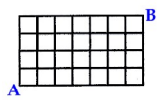
\includegraphics[width=0.2\linewidth]{assets/shortestPath.PNG} 
    
    Jika seseorang akan berjalan dari titik A ke titik B. Ada berapa banyak cara jalan terpendek yang dapat dipilihnya ?

    \item (OSK 2010) Banyaknya himpunan $X$ yang memenuhi 
    $$\{1,2,\dots,1000\} \subseteq X \subseteq \{1,2,\dots,2010\}.$$

    \item (OSP 2010) Bilangan asli enam digit $abcdef$ dengan $a > b > c \ge d > e > f$ ada sebanyak \dots
    
    \item (OSK 2017)
	Sebuah hotel mempunyai kamar bernomor 000 sampai dengan 999. Hotel tersebut menerapkan aturan aneh sebagai berikut: jika suatu kamar berisi tamu, dan sembarang dua digit nomor kamar tersebut dipertukarkan tempatnya, maka diperoleh nomor kamar yang sama atau nomor kamar yang tidak berisi tamu. Maksimal banyaknya kamar yang berisi tamu adalah \dots
\end{enumerate}
\subsection{Permutasi Siklis}
$n$ objek ditaruh mengelilingi lingkaran maka banyak cara menyusunnya adalah
$$P_{siklis} =\dfrac{n!}{n} = (n-1)!$$
\subsection{Latihan Soal Permutasi Siklis}
\begin{enumerate}
    \item (OSK 2013) Enam orang siswa akan duduk pada tiga meja bundar, dimana setiap meja akan diduduki oleh minimal satu siswa. Banyaknya cara untuk melakukan hal tersebut adalah \ldots

    \item (OSK 2015) Suatu sekolah mempunyai lima kelompok belajar siswa kelas 11. Kelompok-kelompok belajar itu berturut-turut mengirimkan 2, 2, 2, 3, dan 3 siswa untuk suatu pertemuan. Mereka akan duduk melingkar sehingga setiap siswa memiliki paling sedikit satu teman dari kelompok belajar yang sama yang duduk di sampingnya. Banyaknya cara melakukan hal tersebut adalah \ldots\\
    (Dua cara mereka duduk melingkar dianggap sama jika salah satu cara dapat diperoleh dari cara yang lain dengan suatu rotasi)
    
\end{enumerate}
\subsection{Stars and Bars}
Banyaknya solusi bulat non-negatif $(x_1,x_2,\dots,x_k)$ dari sistem persamaan $x_1+x_2+\dots+x_k=n$ adalah
$${n+k-1 \choose k-1}.$$
Banyaknya solusi bulat positif $(x_1,x_2,\dots,x_k)$ dari sistem persamaan $x_1+x_2+\dots+x_k=n$ adalah
$${n-1 \choose k-1}.$$
\subsection{Latihan Soal Stars and Bars}
\begin{enumerate}
    \item Carilah banyaknya kuadrupel terurut bilangan ganjil positif $(x_1, x_2, x_3, x_4)$ yang memenuhi $x_1 + x_2 + x_3 + x_4 = 98$.
\end{enumerate}
\subsection{Prinsip Inklusi Eksklusi}
Prinsip Inklusi (memasukkan, dari kata inklusif) Eksklusi (mengeluarkan, khusus, dari kata eksklusif) atau yang sering disingkat PIE, pada dasarnya adalah konsep dari mengurangi "kelebihan hitung" atau menambahkan "kekurangan hitung". Contohnya adalah soal himpunan yang dinyatakan dalam rumus berikut
$$|A \cup B|=|A|+|B|-|A \cap B|.$$

Untuk tiga himpunan $A,B,C$ adalah
$$|A \cup B \cup C|=|A|+|B|+|C|-|A \cap B|-|A \cap C|-|B \cap C|+|A \cap B \cap C|.$$

dan seterusnya. Lebih lengkapnya boleh mengacu ke \href{https://brilliant.org/wiki/principle-of-inclusion-and-exclusion-pie/}{https://brilliant.org/wiki/principle-of-inclusion-and-exclusion-pie/}

\input{High/SubChapter/Combinatorics/derangement}
\subsection{Latihan Soal Prinsip Inklusi Eksklusi}
\begin{enumerate}
    \item (OSK 2017) Terdapat enam anak, $A, B, C, D, E$ dan $F$, akan saling bertukar kado. Tidak ada yang menerima kadonya sendiri, dan kado dari $A$ diberikan kepada $B$. Banyaknya cara membagikan kado dengan cara demikian adalah \dots

    \item (OSK 2023) Banyaknya bilangan 4 digit yang habis dibagi 3 dan memuat angka 6 adalah \ldots
\end{enumerate}
\subsection{Identitas Kombinatorika}
\begin{enumerate}
    \item  ${n \choose k} = {n \choose n-k}$ dengan $k,n \in \NN_0$ dan $k \le n$.
    \item (Identitas Pascal) Untuk $n,k \in \NN_0$ berlaku ${n \choose k} + {n \choose k+1} = {n+1 \choose k+1}$
    \item (Hockey Stick Identity) Untuk $n,r\in\mathbb{N}, n>r,\sum^n_{i=r}{i\choose r}={n+1\choose r+1}$.
    \item Untuk $n,k \in \NN_0$ berlaku ${n \choose 0}+{n \choose 1} + \dots + {n \choose n} = 2^{n}$.
    \item Untuk $n,k \in \NN_0$ berlaku ${n \choose 0}+{n \choose 2} + \dots + {n \choose 2\floor{\frac{n}{2}}} = 2^{n-1}$.
    \item (Vandermonde's Identity)  $\sum_{k=0}^r\binom mk\binom n{r-k}=\binom{m+n}r$
\end{enumerate}
\subsection{Latihan Soal Identitas Kombinatorika}
\begin{enumerate}
    \item (AIME II 2000) Given that
            $\frac 1{2!17!}+\frac 1{3!16!}+\frac 1{4!15!}+\frac 1{5!14!}+\frac 1{6!13!}+\frac 1{7!12!}+\frac 1{8!11!}+\frac 1{9!10!}=\frac N{1!18!}$
            find the greatest integer that is less than $\frac N{100}$. 

        \item (AIME 1986) The polynomial $1-x+x^2-x^3+\cdots+x^{16}-x^{17}$ may be written in the form $a_0+a_1y+a_2y^2+\cdots +a_{16}y^{16}+a_{17}y^{17}$, where $y=x+1$ and the $a_i$'s are constants. Find the value of $a_2$.

        \item (AMC 10A 2016) For some particular value of $N$, when $(a+b+c+d+1)^N$ is expanded and like terms are combined, the resulting expression contains exactly $1001$ terms that include all four variables $a, b,c,$ and $d$, each to some positive power. What is $N$?
\end{enumerate}
\subsection{Binomial Newton}
Binomial Newton atau ekspansi/penjabaran binomial berfokus pada nilai koefisien setiap suku hasil penjabaran $(a+b)^n$.
$$(a+b)^n = {n \choose 0} a^nb^0 + {n \choose 1} a^{n-1}b^1+ \dots +{n \choose n}a^0b^n$$

\subsection{Latihan Soal Ekspansi Binomial Newton}
\begin{enumerate}
    \item Carilah koefisien $x^4$ dari penjabaran $(x+1)^9$

\item (OSK 2013) Koefisien $x^{2013}$ pada ekspansi
$$(1+x)^{4026}+x(1+x)^{4025}+x^2(1+x)^{4024}+\dots x^{2013}(1+x)^{2013}$$
adalah \dots

\item Jika $S=(\sqrt{71}+1)^{71}-(\sqrt{71}-1)^{71}$ adalah bilangan bulat, carilah digit terakhir dari $S$
\end{enumerate}
\subsection{Pigeon Hole Principle (PHP)}
Teorema yang dalam Bahasa Indonesia ini disebut dengan Teorema Sangkar Burung Merpati secara matematis berbunyi:
Jika ada $kn+1$ merpati dan $n$ sangkar, maka setidaknya ada satu sangkar yang berisi $k+1$ burung merpati.

Versi lebih simpelnya adalah: jika ada $n+1$ objek yang akan dibagi ke dalam $n$ buah kotak, maka setidaknya ada 1 kotak yang berisi 2 objek.

Contoh: \begin{itemize}
    \item Di dalam ruangan berisi 3 orang, pasti terdapat setidaknya 2 orang berjenis kelamin sama.
    \item Jika ada 367 orang di suatu sekolah, maka setidaknya ada dua orang diantara mereka yang tanggal lahirnya persis sama.
\end{itemize}
\subsection{Latihan Soal PigeonHole Principle}
\begin{enumerate}
\item Berapa banyak orang minimum yang harus hadir di suatu pesta sehingga dipastikan terdapat 3 orang yang lahir di bulan yang sama di pesta itu?

\item Misalkan Naruko memilih $k$ buah bilangan dari himpunan $\{1,2,3,\dots,2016\}$ secara acak. Berapakah nilai $k$ terkecil sehingga Naruko pasti bisa mendapatkan setidaknya sepasang bilangan (dari $k$ bilangan itu) yang jika dijumlahkan hasilnya 2017?

\item Suatu malam di rumah WonYoung terjadi pemadaman listrik. Karena WonYoung sangat malas, ia hanya ingin tidur dengan membawa banyak kaus kaki (hobi yang aneh :/). Ia mengambil kaus kaki dari lemari di ruangan yang sangat gelap. Lemari itu berisi 100 buah kaus kaki merah, 80 kaus kaki hijau, 60 kaus kaki biru, dan 40 kaus kaki hitam. WonYoung mengambil banyak kaus kaki tapi tidak bisa tahu warnanya. Berapa banyak kaus kaki paling sedikit yang perlu diambil sehingga dijamin terdapat setidaknya 10 pasang kaus kaki (dengan setiap pasang kaus kaki harus berwarna sama) ?

\item (OSK 2011) Di lemari hanya ada 2 macam kaos kaki yaitu kaos kaki berwarna hitam dan putih. Ali, Budi dan Candra berangkat di malam hari saat mati lampu dan mereka mengambil kaos kaki secara acak di dalam lemari dalam kegelapan. Berapa kaos kaki minimal harus mereka ambil untuk memastikan bahwa akan ada tiga pasang kaos kaki yang bisa mereka pakai ? (Sepasang kaos kaki harus memiliki warna yang sama).
    
\item Tandai satu buah kartu dengan angka 1, dua buah kartu dengan angka 2, tiga buah kartu dengan angka satu hingga lima puluh buah kartu dengan angka 50. Semua kartu tersebut dimasukkan ke dalam kotak. Berapa buah kartu minimal yang harus diambil agar dapat dipastikan terdapat sekurang-kurangnya 10 buah kartu dengan tanda angka yang sama 

\item (OSK 2016) Anak laki-laki dan anak perempuan yang berjumlah 48 orang duduk melingkar secara acak. Banyaknya minimum anak perempuan sehingga pasti ada enam anak perempuan yang duduk berdekatan tanpa diselingi anak laki-laki adalah \dots
\end{enumerate}
\subsection{Peluang}
Misalkan kita melempar sekeping koin, maka kegiatan ini disebut dengan percobaan. Hasil percobaan yang didapat biasanya adalah munculnya sisi gambar, $G$, atau munculnya sisi tulisan, $T$. Ruang contoh atau ruang sampel adalah himpunan dari \textbf{semua hasil percobaan yang mungkin} biasanya dilambangkan dengan $S$, yang dalam teori himpunan disebut dengan himpunan semesta. Pada percobaan melempar koin, ruang sampelnya adalah $\{G, T\}$ sedangkan pada percobaan melempar satu buah dadu, ruang sampelnya adalah $\{1, 2, 3, 4, 5, 6\}$. Jika $\{G, T\}$ adalah ruang sampel, maka anggota-anggota dari ruang sampel tersebut disebut titik contoh. Titik contoh dari $\{G, T\}$ adalah $G$ dan $T$. Pada percobaan melempar satu buah dadu seimbang, titik sampel yang didapat ada 6 yaitu 1, 2, 3, 4, 5, 6 sedangkan jika melempar dua buah dadu akan didapat 36 buah titik contoh, yaitu $(1, 1), (1, 2), (1, 3), \dots , (6, 6)$. 

\subsubsection{Formula Penghitungan Peluang}
Secara mudahnya, enghitung peluang bisa dengan pendekatan frekuensi, yaitu suatu percobaan yang dilakukan sebanyak $n$ kali, ternyata kejadian $A$ munculnya sebanyak $k$ kali, maka frekuensi nisbi/relatif kejadian $A$ sama dengan 
$$p(A)=\dfrac{k}{n}$$
Kalau $n$ semakin besar dan menuju tak terhingga maka nilai $p(A)$ akan cenderung konstan mendekati suatu nilai tertentu yang disebut dengan peluang munculnya kejadian $A$.

\subsection{Latihan Soal Peluang}
\begin{enumerate}
        \item (OSK 2015) Suatu dadu ditos enam kali. Probabilitas jumlah mata dadu yang muncul 9 adalah \ldots

        \item (OSK 2012) Suatu set soal terdiri dari 10 soal pilihan B atau S dan 15 soal pilihan ganda dengan 4 pilihan. Seorang siswa menjawab semua soal dengan menebak jawaban secara acak. Tentukan probabilitas ia menjawab dengan benar hanya 2 soal.

        \item (OSK 2013) Suatu partikel bergerak pada bidang Cartesius dari titik $(0, 0)$. Setiap langkah bergerak satu satuan searah sumbu $X$ positif dengan probabilitas $0.6$ atau searah sumbu $Y$ positif dengan probabilitas $0.4$. Setelah sepuluh langkah, probabilitas partikel tersebut sampai pada titik $(6,4)$ dengan melalui titik $(3,4)$ adalah \ldots
        
        \item (OSK 2012) Misalkan terdapat 5 kartu dimana setiap kartu diberi nomor yang berbeda yaitu 2, 3, 4, 5, 6. Kartu-kartu tersebut kemudian dijajarkan dari kiri ke kanan secara acak sehingga berbentuk barisan. Berapa probabilitas bahwa semua kartu yang dijajarkan dari kiri ke kanan dan ditempatkan pada tempat ke- $i$ akan lebih besar atau sama dengan $i$ untuk setiap $i$ dengan $1 \le i \le 5$ ?
        
        \item (OSK 2013) Suatu dadu ditos enam kali. Banyak cara memperoleh jumlah mata yang muncul 28 dengan tepat satu dadu muncul angka 6 adalah \dots
        
        \item (OSK 2013) Sepuluh kartu ditulis dengan angka satu sampai sepuluh (setiap kartu hanya terdapat satu angka dan tidak ada dua kartu yang memiliki angka yang sama). Kartu - kartu tersebut dimasukkan kedalam kotak dan diambil satu secara acak. Kemudian sebuah dadu dilempar. Probabilitas dari hasil kali angka pada kartu dan angka pada dadu menghasilkan bilangan kuadrat adalah \dots
        
        \item (OSK 2018) Diberikan satu koin yang tidak seimbang. Bila koin tersebut ditos satu kali, peluang muncul angka adalah $\frac{1}{4}$. Jika ditos $n$ kali, peluang muncul tepat dua angka sama dengan peluang muncul tepat tiga angka. Nilai $n$ adalah \dots
        
        \item (OSK 2017) Pada suatu kotak ada sekumpulan bola berwarna merah dan hitam yang secara keseluruhannya kurang dari 1000 bola. Misalkan diambil dua bola. Peluang terambilnya dua bola merah adalah $p$ dan peluang terambilnya dua bola hitam adalah $q$ dengan $p-q =\frac{23}{37}$. Selisih terbesar yang mungkin dari banyaknya bola merah dan hitam adalah \dots
\end{enumerate}
\subsection{Relasi Rekurensi}
Sering disebut dengan rekursif. Intinya adalah sebuah persamaan yang melibatkan barisan $a_1, a_2, \dots , a_n$ dimana untuk mendapatkan nilai $a_k$ membutuhkan suku-suku sebelumnya $a_{k-1}, a_{k-2}, \dots,$ atau $a_1$. 

Contoh paling terkenal dari persamaan rekursif adalah bilangan Fibonacci $0,1,1,2,3,5,8,13,21,\dots$ yang secara matematis didefinisikan sebagai berikut.
\begin{align*}
    F_0 &= 0, F_1 = 1\\
    F_n &= F_{n-1}+F_{n-2} \text{ untuk } n \ge 2
\end{align*}

atau yang lebih terkenal di ranah \textit{Computer Science} adalah permasalahan \textit{Tower of Hanoi} dengan persamaan rekursifnya didefinisikan sebagai berikut.
\begin{align*}
    T_1 &= 1 \\
    T_n &= 2T_{n-1}+1
\end{align*}

Untuk menyelesaikan soal relasi rekurensi, butuh manipulasi aljabar yang mumpuni sehingga tidak ada pendekatan eksplisit selain menggunakan persamaan karakteristik atau fungsi pembangkit (tidak dibahas disini) yang dijamin berhasil.

\input{High/SubChapter/Combinatorics/persamaanKarakteristikRekursif}
\subsection{Latihan Soal Relasi Rekurensi}
\begin{enumerate}
    \item (British) Isaac is planning a nine-day holiday. Every day he will go surfing, or water skiing, or he will rest. On any given day he does just one of these three things. He never does different water-sports on consecutive days. How many schedules are possible for the holiday?

    \item (AIME I 2006) A collection of 8 cubes consists of one cube with edge-length $k$ for each integer $k, 1 \le k \le 8.$ A tower is to be built using all 8 cubes according to the rules:
    \begin{itemize}
        \item Any cube may be the bottom cube in the tower.
        \item The cube immediately on top of a cube with edge-length $k$ must have edge-length at most $k+2.$
    \end{itemize}
    Let $T$ be the number of different towers than can be constructed. What is the remainder when $T$ is divided by 1000?

    \item (AIME I 2006) For each even positive integer $x$, let $g(x)$ denote the greatest power of 2 that divides $x.$ For example, $g(20)=4$ and $g(16)=16.$ For each positive integer $n,$ let $S_n=\sum_{k=1}^{2^{n-1}}g(2k).$ Find the greatest integer $n$ less than 1000 such that $S_n$ is a perfect square.

    \item (AIME I 2001) A mail carrier delivers mail to the nineteen houses on the east side of Elm Street. The carrier notices that no two adjacent houses ever get mail on the same day, but that there are never more than two houses in a row that get no mail on the same day. How many different patterns of mail delivery are possible?
\end{enumerate}
\section{Geometri}
Pada dasarnya geometri di olimpiade matematika SMA "hanya" tentang lingkaran dan segitiga dua dimensi (Soal bangun tiga dimensi hampir ngga pernah dikeluarin untuk lomba tingkat SMA).
\subsection{Garis, Segmen Garis, Sinar (Bukan Vektor!)}
    Perlu ditekankan bahwa \textbf{garis tidak sama dengan ruas garis}. Garis panjangnya tak hingga, sedangkan ruas garis atau segmen garis panjangnya terbatas. Gambar di bawah terdiri dari \textbf{garis AB, segmen garis CD, sinar EF}.
\begin{center}
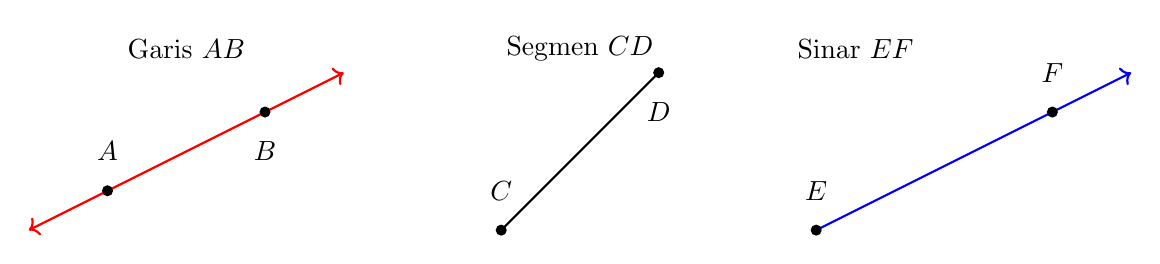
\begin{tikzpicture}
    % Draw a line
    \draw[red, thick, <->] (-4,-1) -- (0,1);
    \node at (-2,1.3) {Garis $AB$};
    \fill (-3,-0.5) circle (2pt);
    \fill (-1,0.5) circle (2pt);
    \node at (-3,-0) {$A$};
    \node at (-1,0) {$B$};

    % Draw a segment
    \draw[thick] (2,-1) -- (4,1);
    \node at (3,1.3) {Segmen $CD$};
    \fill (2,-1) circle (2pt);
    \fill (4,1) circle (2pt);
    \node at (2,-0.5) {$C$};
    \node at (4,0.5) {$D$};

    % Draw a ray
    \draw[blue, thick, ->] (6,-1) -- (10,1);
    \node at (6.5,1.3) {Sinar $EF$};
    \fill (6,-1) circle (2pt);
    \fill (9,0.5) circle (2pt);
    \node at (6,-0.5) {$E$};
    \node at (9,1) {$F$};
\end{tikzpicture}
\end{center}
\subsection{Lingkaran}

\begin{center}
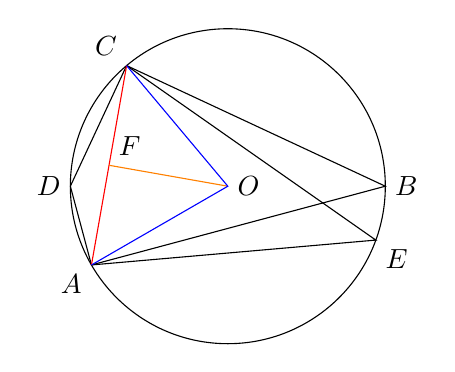
\begin{tikzpicture}
\coordinate (O) at (0,0);
\coordinate (B) at (0:2cm);
\coordinate (A) at (210:2cm);
\coordinate (D) at (180:2cm);
\coordinate (C) at (130:2cm);
\coordinate (E) at (-20:2cm);

\draw (O) circle (2cm);

\draw (A) -- (B) -- (C) -- (D) -- cycle;
\draw (A) -- (E) -- (C);
\draw[red] (A) -- (C);

\tkzDefPointBy[projection=onto A--C](O) \tkzGetPoint{F}
\draw[orange] (O) -- (F);
\draw[blue] (C) -- (O) -- (A);

\node[right] at (B) {$B$};
\node[below left] at (A) {$A$};
\node[left] at (D) {$D$};
\node[above left] at (C) {$C$};
\node[below right] at (E) {$E$};
\node[right] at (O) {$O$};
\node[above right] at (F) {$F$};
\end{tikzpicture}
\end{center}

    
Misalkan $O$ pusat lingkaran $\Gamma$ dan $A,B,C,D,E$ adalah sembarang titik pada lingkaran $\Gamma$ seperti pada gambar.
\begin{enumerate}
    \item $CO=OA$ adalah jari-jari dengan $\angle ACO = \angle OAC$.
    \item Misalkan titik $F$ adalah titik tengah tali busur $CA$, maka $OF \perp CA$ atau $OF$ tegak lurus dengan $CA$, dengan kata lain, $F$ adalah proyeksi titik $O$ ke $CA$
    \item (Sudut keliling-sudut pusat) Untuk$\angle COA = 2\angle CBA$.
    \item (sudut keliling) $\angle CBA = \angle CEA$.
    \item $ABCD$ adalah segiempat tali busur atau segiempat siklis  atau $A,B,C,D$ terletak di lingkaran (seperti pada gambar) jika dan hanya jika $\angle CBA + \angle ADC = 180^\circ$ atau $\angle ABD = \angle ACD$.
\end{enumerate}
\subsection{Latihan Soal Lingkaran}
\begin{enumerate}
    \item Pada segiempat $WXYZ$ dengan diagonal yang saling tegak lurus diketahui bahwa $\angle WZX = 30^\circ, \angle XWY = 40^\circ,$ and $\angle WYZ = 50^\circ$. Hitunglah besar $\angle X$ dan $\angle Z$.
    \begin{center}
        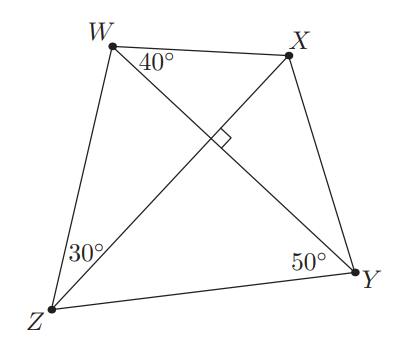
\includegraphics[width=0.25\textwidth]{assets/evanquad.PNG}
    \end{center}
		
    \item (OSK 2013) Diberikan segitiga lancip $ABC$ dengan $O$ sebagai pusat lingkaran luarnya. Misalkan $M$ dan $N$ berturut - turut pertengahan $OA$ dan $BC$. Jika $\angle ABC = 4\angle OMN$ dan $\angle ACB = 6\angle OMN$, maka besarnya $\angle OMN$ sama dengan \dots

    \item 	Pada gambar di bawah, diketahui titik A $\ne$ B pada lingkaran berdiameter $MN$ dan berpusat di $C$. $P$ adalah titik pada segmen $CN$ dimana $\angle CAP = \angle CBP = 10 ^\circ$. Jika $\angle ACM = 40^\circ$, maka $\angle BCN = \dots^\circ$	
    \begin{center}
         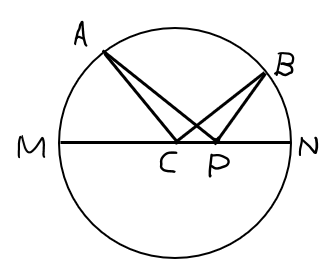
\includegraphics[width=0.25\textwidth]{assets/soalLingkaran1.PNG}
    \end{center}

    \item (OSK 2011,2012,2013,2018) Diberikan segitiga $ABC$ dan lingkaran $\Gamma$ yang berdiameter $AB$. Lingkaran $\Gamma$ memotong sisi $AC$ dan $BC$ berturut-turut di titik $D$ dan $E$. Jika $AD = \frac13 AC, BE =\frac14 BC$ dan $AB = 30$, maka luas segitiga $ABC$ adalah \dots

    \item (OSK 2015) Diberikan segitiga $ABC$ dengan sudut $\angle ABC = 90^\circ$. Lingkaran $L_1$ dengan $AB$ sebagai diameter sedangkan lingkaran $L_2$ dengan $BC$ sebagai diameternya. Kedua lingkaran $L_1$ dan $L_2$ berpotongan di $B$ dan $P$. Jika $AB = 5$, $BC = 12$ dan $BP = x$ maka nilai dari $\frac{240}{x}$ adalah \ldots
\end{enumerate}
\subsection{Segitiga}
Pada segitiga $ABC$ seperti gambar berikut:
\begin{center}
\begin{tikzpicture}
    % Define the coordinates of the vertices
    \coordinate (A) at (0,0);
    \coordinate (B) at (8,0);
    \coordinate (C) at (1.5,4);
    
    % Draw the triangle
    \draw (A) -- (B) -- (C) -- cycle;
    
    % circumcircle
    \tkzCircumCenter(A,B,C)\tkzGetPoint{O}
    \tkzDrawPoint(O)
    \tkzDrawCircle(O,A)
    
    % incircle
    \tkzDefCircle[in](A,B,C)\tkzGetPoint{I}\tkzGetLength{rIN}
    \tkzDrawPoint(I)
    \tkzDrawCircle[R](I,\rIN pt)
    
    % angle bisector
    \tkzDrawBisector[blue](B,A,C)\tkzGetPoint{E}
    \tkzDrawCircle[R](E,1 pt)
    
    %altitude
    \tkzDefPointBy[projection=onto B--C](A) \tkzGetPoint{D}
    \tkzDefPointBy[projection=onto B--A](C) \tkzGetPoint{C1}
    \tkzInterLL(A,D)(C,C1) \tkzGetPoint{H}
    \tkzDrawPoints(H) \tkzLabelPoints[below right](H)
    \tkzDrawSegment[red](A,D)
    \tkzDrawSegment[red](C,C1)

    %garis sumbu
    \tkzDefPointBy[projection=onto B--C](O) \tkzGetPoint{M}
    \tkzDefPointBy[homothety=center O ratio 3.2](M) \tkzGetPoint{M1}
    \tkzDefPointBy[homothety=center O ratio -3.2](M) \tkzGetPoint{M2}
    \tkzDrawSegment(M1,M2)
    \tkzDefPointBy[projection=onto B--A](O) \tkzGetPoint{M3}

    %centroid
    \tkzDrawSegment[green](A,M)
    \tkzDrawSegment[green](C,M3)
    \tkzInterLL(A,M)(C,M3) \tkzGetPoint{G}
    \tkzDrawPoints(G) \tkzLabelPoints[below right](G)
    
    % Label the vertices
    \node[below left] at (A) {$A$};
    \node[below right] at (B) {$B$};
    \node[above] at (C) {$C$};
    \node[below right] at (I) {$I$};
    \node[right] at (O) {$O$};
    \node[above right] at (E) {$E$};
    \node[above] at (D) {$D$};
    \node[right] at (M) {$M$};
\end{tikzpicture}
\end{center}
\begin{enumerate}
    \item Garis bagi $AE$ yaitu garis yang membagi dua sudut $A$ sama besar sehingga $\angle BAE = \angle EAC$. 
    \item Garis berat $AM$ dengan $M$ adalah titik tengah $BC$.
    \item Garis tinggi $AD$ adalah garis yang tegak lurus dengan $BC$. $D$ biasa disebut dengan proyeksi $A$ ke $BC$.
    \item Garis $OM$ adalah salah satu garis sumbu segitiga $ABC$, yaitu garis yang melewati titik tengah sisi segitiga dan tegak lurus dengan sisi itu.
    \item Pertemuan atau perpotongan ketiga garis tinggi segitiga $ABC$ adalah titik tinggi, dalam gambar ini adalah $H$ (orthocenter).
    \item Pertemuan atau perpotongan ketiga garis bagi segitiga $ABC$ adalah titik bagi atau titik pusat lingkaran dalam (incircle) segitiga $ABC$ dalam gambar ini adalah $I$ (incenter).
    \item Pertemuan atau perpotongan ketiga garis berat segitiga $ABC$ adalah titik berat (centroid).
    \item Pertemuan atau perpotongan ketiga garis sumbu segitiga $ABC$ adalah titik pusat lingkaran luar (circumcircle) segitiga $ABC$ yang dalam gambar ini adalah $O$ (circumcenter).
    \item Berlaku \textbf{ketaksamaan segitiga} yaitu $AB+BC>CA$, $BC+CA>AB$, dan $CA+AB>BC$. Selain itu juga berlaku $|AB-BC|<CA$, $|BC-CA|<AB$, dan $|CA-AB|<BC$.
\end{enumerate}
\input{High/SubChapter/Geometry/segitigaSebangunKongruen}
\input{High/SubChapter/Geometry/pythagoras}
\subsection{Latihan Soal Segitiga }
\begin{enumerate}    
    \item Garis berat $AD$ pada segitiga $ABC$ memotong garis berat $CF$ di titik $P$, serta perpanjangan $BP$ memotong $AC$ di $E$. Jika diketahui segitiga $ABC$ lancip dan $AB=6$, maka panjang $DE$ adalah \dots

    \item (OSK 2011,2012,2013,2018) Diberikan segitiga $ABC$ dan lingkaran $\Gamma$ yang berdiameter $AB$. Lingkaran $\Gamma$ memotong sisi $AC$ dan $BC$ berturut-turut di titik $D$ dan $E$. Jika $AD = \frac13 AC, BE =\frac14 BC$ dan $AB = 30$, maka luas segitiga $ABC$ adalah \dots
		
    \item Diberikan segitiga $ABC$ dengan $D$ titik tengah $AC$, $E$ titik tengah $BD$, dan $H$ merupakan pencerminan $A$ terhadap $E$. Jika $F$ merupakan perpotongan antara $AH$ dengan $BC$, maka nilai $\dfrac{AF}{FH}$ sama dengan \dots
		 
    \item Diberikan segitiga $ABC$ dengan panjang sisi $BC = 20$, $CA = 24$, dan $AB=12$. Titik $D$ pada segmen $BC$ dengan $BD = 5$. Lingkaran luar dari segitiga $ABD$ memotong $CA$ di $E$. Hitunglah nilai $2 \times DE$.

    \item (OSK 2015) Diberikan trapesium $ABCD$ dengan $AB$ sejajar $DC$ dan $AB = 84$ serta $DC = 25$. Jika trapesium $ABCD$ memiliki lingkaran dalam yang menyinggung keempat sisinya, keliling trapesium $ABCD$ adalah \ldots

    \item (OSK 2022) Diberikan segitiga siku-siku $ABC$. Jika luas dari segitiga $ABC$ adalah 112. Misalkan $R$ adalah panjang jari-jari lingkaran luar segitiga $ABC$ dan $r$ adalah panjang jari-jari lingkaran dalam segitiga $ABC$. Diketahui juga $R + r = 16$. Panjang sisi miring dari segitiga $ABC$ adalah \ldots
\end{enumerate}
\subsection{Latihan Soal Pythagoras}
\begin{enumerate}
    \item (OSK SMP 2016) Diketahui $ABCD$ dan $CEGH$ adalah dua persegipanjang kongruen dengan panjang $17$ cm, dan lebar $8$ cm. Titik $E$ berada di sisi $AB$ dan $D$ berada di sisi $GH$. Titik $F$ adalah titik potong sisi $AD$ dan $EG$. Luas segiempat $EFDC$ adalah .... $cm^2$.

    \item Misalkan $ABC$ adalah segitiga lancip. Titik $D$, $E$, dan $F$ terletak pada sisi $BC$, $CA$, dan $AB$, berturut-turut, sedemikian sehingga $AD$, $BE$, dan $CF$ adalah garis tinggi segitiga $ABC$. Titik $H$ adalah titik tinggi segitiga $ABC$. Jika $DE = 8$, $DF = 15$, dan $EF = 17$, tentukan panjang $AH$.

    \item (OSK 2015) Diberikan segitiga $ABC$ dengan sudut $\angle ABC = 90^\circ$. Lingkaran $L_1$ dengan $AB$ sebagai diameter sedangkan lingkaran $L_2$ dengan $BC$ sebagai diameternya. Kedua lingkaran $L_1$ dan $L_2$ berpotongan di $B$ dan $P$. Jika $AB = 5$, $BC = 12$ dan $BP = x$ maka nilai dari $\frac{240}{x}$ adalah \ldots

    \item (OSK 2022) Diberikan segitiga $ABC$ siku-siku di B. Titik $D$ berada pada sisi $AB$ dan titik $E$ berada pada sisi $AC$. Diketahui $DE$ sejajar $BC$. Jika $AD = 21$, $DB = 3$, dan $BC = 32$, maka panjang $AE$ adalah \dots

\end{enumerate}
\subsection{Power of a point}
\begin{figure}[h]
  \begin{asy}
    unitsize(1.5cm);
    pair O, A, B, C, D, E, P;
    O = (0,0);
    P = (4,1);
    E = (0,1);
    A = dir(50);
    C = dir(-30);
    circle o = circumcircle(A,E,C);
    draw(o);
    pair B1[] = intersectionpoints(line(A,P), o);
    pair D1[] = intersectionpoints(line(C,P), o);
    B = B1[0];
    D = D1[0];
    draw(A--B);
    draw(C--D);
    draw(P--A);
    draw(P--D);
    draw(P--E, red);
    draw(P--O, blue+dotted);
    label("$O$",O,SW);
    label("$A$",A,E);
    label("$B$",B,N);
    label("$C$",C,SE);
    label("$D$",D,SW);
    label("$P$",P,NE);
    label("$E$",E,N);
    \end{asy}
    \begin{asy}
    unitsize(1.5cm);
    pair O, A, B, C, D, P;
    O = (0,0);
    A = dir(50);
    C = dir(130);
    D = dir(-30);
    B = dir(-110);
    P = extension(A,B,C,D);
    draw(circumcircle(A,B,C));
    draw(A--B);
    draw(C--D);
    draw(A--C--B--D--cycle);
    draw(O--P, dotted);
    label("$O$",O,SW);
    label("$A$",A,E);
    label("$B$",B,SW);
    label("$C$",C,NW);
    label("$D$",D,SE);
    label("$P$",P,E);
    \end{asy}
\end{figure}
Diberikan lingkaran $\Gamma$ dan titik $P$ yang terletak di dalam atau di luar lingkaran $\Gamma$. Maka definisikan kuasa atau power dari $P$ terhadap lingkaran $\Gamma$ sebagai
$$Pow_\Gamma (P) = |OP^2-r^2|$$
dimana $O$ adalah pusat dari $\Gamma$ dan $r$ adalah jari-jari lingkaran $\Gamma$.

Jika $A,B,C,D$ berada di $\Gamma$, serta $AB$ dan $CD$ berpotongan di $P$, maka $$Pow_\Gamma(P)=PA \cdot PB = PC \cdot PD.$$
Jika $P$ berada di luar $\Gamma$ dan $E$ berada di $\Gamma$ sehingga $PE$ bersinggungan dengan $\Gamma$ di $E$, maka $$Pow_\Gamma (P) = PE^2 =  PA \cdot PB = PC \cdot PD.$$
\subsection{Latihan Soal Power of A Point}
\begin{enumerate}
    \item (\textbf{Soal Legend: OSK 2011,2012,2013,2018}) Diberikan segitiga $ABC$ dan lingkaran $\Gamma$ yang berdiameter $AB$ . Lingkaran $\Gamma$ memotong sisi $AC$ dan $BC$ berturut-turut di titik $D$ dan $E$. Jika $AD = \frac13 AC, BE =\frac14 BC$ dan $AB = 30$, maka luas segitiga $ABC$ adalah \dots

    \item (OSN SL 2010) Pada segitiga $ABC$, misalkan $D$ adalah titik tengah $BC$, dan $BE$, $CF$ adalah garis tinggi. Buktikan bahwa $DE$ dan $DF$ keduanya adalah garis singgung lingkaran luar $\triangle AEF$. %(OSN SL 2010) 

    %AIME 2016 I and AIME 2016 I
    \item (AIME 2016 I) Misalkan $\triangle ABC$ adalah segitiga lancip dengan lingkaran $\omega,$ dan misalkan $H$ adalah titik potong dari garis tinggi $\triangle ABC.$ Garis singgung lingkaran luar $\triangle HBC$ di $H$ memotong $\omega$ pada titik $X$ dan $Y$ dengan $HA=3,HX=2,$ dan $HY=6.$ Carilah luas dari $\triangle ABC$.

    \item (AIME 2016 I) Lingkaran $\omega_1$ dan $\omega_2$ bertemu di titik $X$ dan $Y$. Garis $\ell$ menyinggung lingkaran $\omega_1$ dan $\omega_2$ di $A$ dan $B$, berturut-turut, dengan garis $AB$ lebih dekat ke titik $X$ daripada $Y$. Lingkaran $\omega$ yang melewati $A$ dan $B$, memotong $\omega_1$ lagi di $D \neq A$ dan memotong $\omega_2$ lagi di $C \neq B$. Ketiga titik $C$, $Y$, $D$ segaris dengan $XC = 67$, $XY = 47$, dan $XD = 37$. Carilah panjang $AB$.
\end{enumerate}
\subsection{Trigonometri}
Banyak sih rumusnya, tapi yang paling sering dipake di olim:
\begin{enumerate}
    \item $\sin (-x) = -\sin x$.
    \item $\cos (-x) = \cos x$.
    \item $\tan(-x) = -\tan x$.
    \item $\sin (90^\circ-x) = \sin(90^\circ+x)=\cos x$
    \item $\sin^2 x + \cos^2 x = 1$.
    \item $\sin(90^\circ-x)=\sin(90^\circ+x)=\cos x$.
    \item $\sin(a \pm b) = \sin a \cos b \pm \cos a \sin b$.
    \item $\sin 2x = 2\sin x \cos x$.
    \item $\cos(a \pm b) = \cos a \cos b \mp \sin a \sin b$.
    \item $\cos 2x = \cos^2 x - \sin^2 x = 2\cos^2 x -1 = 1-2\sin^2 x$.
    \item $\tan(a \pm b) = \dfrac{\tan a \pm \tan b}{1 \mp \tan a \tan b}$.
\end{enumerate}
Cara menghafal yang gampang bisa pake "metode sumbu".
\subsection{Latihan Soal Trigonometri}
\begin{enumerate}
    \item (OSK 2022) Diberikan segitiga $ABC$ seperti di gambar, dengan panjang $AB = 2BC$ dan $BD = CD$. Jika luas segitiga $DEC$ adalah 10, luas dari segitiga $AFE$ adalah \dots

	\item Jika $A+B=45^\circ$ dan $\cos A\sin B=\frac{\sqrt{2}}{6}$, maka $\cos(B-A)=\dots$
	
	\item Nilai dari $\cos \dfrac{\pi}{7}\cdot \cos \dfrac{2\pi}{7} \cdot \cos \dfrac{4\pi}{7}$ adalah \dots
	
	\item Pada segitiga $ABC$, buktikan bahwa $\tan A + \tan B + \tan C = \tan A \tan B \tan C$.
	
	\item Tentukan nilai eksak dari $\tan 1^\circ \cdot \tan 2^\circ \cdot \tan 3^\circ \cdot \ldots \cdot \tan 89^\circ$.
	
	\item (OSK 2005) Nilai dari $\sin^8 75^\circ - \cos^8 75^\circ$ adalah \dots
\end{enumerate}
\subsection{Segi-n}
Pada segi-$n$, jumlah sudut totalnya adalah $(n-2)\times 180^\circ$. Hal ini dikarenakan kita dapat membuat $n-2$ segitiga di dalam sembarang segi-$n$ dimana jumlah total sudut dalam setiap segitiga adalah $180^\circ$.\\

Dari fakta tersebut, berarti besar setiap sudut segi-$n$ beraturan adalah $\dfrac{(n-2)}{n}180^\circ$.


\subsection{Luas}
Misalkan $[A_1A_2A_3\dots A_n]$ menotasikan luas bangun $A_1A_2A_3\dots A_n$. 

Misalkan $r$ adalah panjang jari-jari lingkaran dalam $\triangle ABC$, $s=\frac{1}{2}(a+b+c)$ adalah setengah keliling $\triangle ABC$ dimana $a=BC, b=CA, c=AB$ serta $AT$ adalah garis tinggi $\triangle ABC$.

\input{High/SubChapter/Geometry/perbandinganLuas}
\input{High/SubChapter/Geometry/luasSegitigaStandar}
\input{High/SubChapter/Geometry/luasSegitigaTrigon}
\input{High/SubChapter/Geometry/luasSegitigaInradius}
\input{High/SubChapter/Geometry/luasSegitigaCircumradius}
\input{High/SubChapter/Geometry/rumusHeron}

\subsection{Latihan Soal Luas}
\begin{enumerate}
\item (OSK 2006) Pada segitiga $ABC$, titik $F$ membagi sisi $AC$ dalam perbandingan $1 : 2$. Misalkan $G$ titik tengah $BF$ dan $E$ titik perpotongan antara sisi $BC$ dengan $AG$. Maka titik $E$ membagi sisi $BC$ dalam perbandingan \dots

\item (OSK 2009) Diberikan persegi $ABCD$ dengan panjang sisi 10. Misalkan $E$ pada $AB$ dan $F$ pada $BC$ dengan $AE = FB = 5$. Misalkan $P$ adalah titik potong $DE$ dan $AF$. Luas $DCFP$ adalah \dots

\item Pada segitiga $ABC$, titik $D$ dan $E$ berturut-turut berada di segmen $AB$ dan $AC$. Misalkan $CD$ dan $BE$ berpotongan di titik $F$. Jika $[DBF]=3$, $[BFC]=6$, dan $[CFE]=4$, berapakah luas $ADFE$?

\item (OSK 2016) Pada segitiga ABC, titik $X, Y$ dan $Z$ berturut-turut terletak pada sinar $BA, CB$ dan $AC$ sehingga $BX = 2BA, CY = 2CB$ dan $AZ = 2AC$. Jika luas segitiga $ABC$ adalah 1, maka luas segitiga $XYZ$ adalah \dots

\item (OSK 2016) Segitiga $ABC$ merupakan segitiga sama kaki dengan panjang $AB = AC = 10 $. Titik $D$ terletak pada garis $AB$ sejauh $7 $ dari $A$ dan $E$ titik pada garis $AC$ yang terletak sejauh $4 $ dari $A$. Dari $A$ ditarik garis tinggi dan memotong $BC$ di $F$. Jika bilangan rasional $\frac{a}{b}$ menyatakan perbandingan luas segi empat $ADFE$ terhadap luas segitiga $ABC$ dalam bentuk yang paling sederhana, maka nilai $a + b$ adalah \dots

\item (OSK 2014) Diberikan segitiga $ABC$ yang sisi-sisinya tidak sama panjang sehingga panjang garis berat $AN$ dan $BP$ berturut-turut 3 dan 6. Jika luas segitiga $ABC$ adalah $3\sqrt{15}$, maka panjang garis berat ketiga $CM$ adalah \dots

\item (OSK 2012) Diketahui $\triangle ABC$ sama kaki dengan panjang $AB = AC = 3$, $BC = 2$, titik $D$ pada sisi $AC$ dengan panjang $AD = 1$. Tentukan luas $\triangle ABD$.

\item (OSK 2012) Diberikan segitiga $ABC$ dengan keliling 3, dan jumlah kuadrat sisi-sisinya sama dengan 5. Jika jari-jari lingkaran luarnya sama dengan 1, maka jumlah ketiga garis tinggi dari segitiga $ABC$ tersebut adalah \dots

\item (OSN 2011 SMP/MTs) Bangun datar $ABCD$ adalah trapesium dengan $AB$ sejajar $CD$ dan $AB < CD$. Titik $E$ dan $F$ terletak ada $CD$ sehingga $AD$ sejajar $BE$ dan $AF$ sejajar $BC$. Titik $H$  adalah perpotongan $AF$ dengan $BE$ dan titik $G$ adalah  perpotongan $AC$ dengan $BE$. Jika panjang $AB$ adalah 4 cm dan panjang $CD$ adalah 10 cm hitunglah perbandingan luas  segitiga $AGH$ dengan luas trapesium $ABCD$. 
\end{enumerate}
\subsection{Teorema Garis Bagi}
Misalkan garis bagi sudut $\angle A$ (bisa garis bagi dalam atau garis bagi luar) memotong garis $BC$ di $K$, maka 
$$\dfrac{BK}{CK} = \dfrac{AB}{AC}.$$
\begin{center}
    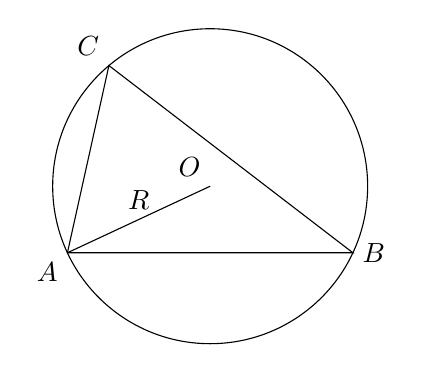
\begin{tikzpicture}
        \coordinate (O) at (0,0);
        \coordinate (B) at (-25:2cm);
        \coordinate (A) at (205:2cm);
        \coordinate (C) at (130:2cm);
        \coordinate (D) at (-90:2cm);
        
        \draw (O) circle (2cm);
        \draw (A) -- (B) -- (C) -- cycle;
        \node[right] at (B) {$B$};
        \node[below left] at (A) {$A$};
        \node[above left] at (C) {$C$};
        \node[above left] at (O) {$O$};
        \draw (A) -- node[above]{$R$} (O);
    \end{tikzpicture}
\end{center}
\subsection{Latihan Soal Teorema Garis Bagi}
\begin{enumerate}
    \item (OSK 2014) Diberikan segitiga $ABC$ dengan $AB = 360, BC = 240,$ dan $AC = 180$. Garis bagi dalam dan garis bagi luar dari $\angle CAB$ memotong $BC$ dan perpanjangan $BC$ berturut-turut di $P$ dan $Q$. Jari-jari lingkaran yang melalui titik-titik $A, P,$ dan $Q$ adalah \dots
    
    \item (OSK 2015) Pada segitiga $ABC$, garis tinggi $AD$, garis bagi $BE$ dan garis berat $CF$ berpotongan di satu titik. Jika panjang $AB = 4$ dan $BC = 5$, dan $CD = \frac{m^2}{n^2}$ dengan $m$ dan $n$ relatif prima, maka nilai dari $m - n$ adalah \ldots
\end{enumerate}
\subsection{Dalil Sinus dan Dalil Cosinus}
    Misalkan $ABC$ adalah suatu segitiga dengan $R$ adalah panjang jari-jari lingkaran luarnya.
\begin{center}
    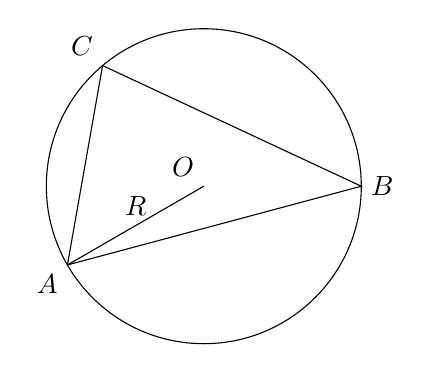
\begin{tikzpicture}
    \coordinate (O) at (0,0);
    \coordinate (B) at (0:2cm);
    \coordinate (A) at (210:2cm);
    \coordinate (C) at (130:2cm);
    
    \draw (O) circle (2cm);
    \draw (A) -- (B) -- (C) -- cycle;
    \node[right] at (B) {$B$};
    \node[below left] at (A) {$A$};
    \node[above left] at (C) {$C$};
    \node[above left] at (O) {$O$};
    \draw (A) -- node[above]{$R$} (O);
    \end{tikzpicture}
\end{center}
    \subsubsection{Dalil Sinus}
    $$\dfrac{BC}{\sin \angle A} = \dfrac{CA}{\sin \angle B}= \dfrac{AB}{\sin \angle C} = 2R$$
    
    \subsubsection{Dalil Cosinus}
    \begin{align*}
        AB^2 &= BC^2 + CA^2 - 2\cdot BC \cdot CA \cdot \cos \angle C\\
        BC^2 &= CA^2 + AB^2 - 2\cdot CA \cdot AB \cdot \cos \angle A\\
        CA^2 &= AB^2 + BC^2 - 2\cdot AB \cdot BC \cdot \cos \angle B
    \end{align*}
\subsection{Latihan Soal Dalil Sinus dan Cosinus}
\begin{enumerate}
    \item (OSK 2016) Pada segitiga $ABC$, titik $M$ terletak pada $BC$ sehingga $AB=7, AM=3, BM=5$, dan $MC=6$. Panjang $AC$ adalah \dots

    \item (OSK 2013) Misalkan $P$ adalah titik interior dalam daerah segitiga $ABC$ sehingga besar $\angle PAB = 10^\circ, \angle PBA = 20^\circ, \angle PCA = 30^\circ, \angle PAC=40^\circ$. Besar $\angle ABC = \dots$
    
    \item (LMNAS SMP 33 Penyisihan) Diberikan segitiga tumpul $ABC$ dengan $AB = BC$. Titik $D$ berada di dalam segitiga tersebut sedemikian sehingga $AD = BD$, $\angle ADB = 140^\circ$, dan $\angle ADC = 150^\circ$. Besar sudut $ACD$ dalam satuan $^\circ$ (derajat) adalah \dots
    
    \item (Modifikasi OSK 2017) Pada sebuah lingkaran dengan pusat $O$, talibusur $AB$ berjarak 5 dari titik $O$ dan talibusur $AC$ berjarak $5\sqrt{2}$ dari titik $O$ dengan titik $A$ terletak di busur $BC$ yang lebih kecil ($A$ diantara $B$ dan $C$) Jika panjang jari-jari lingkaran 10, maka $BC^2=\dots$
\end{enumerate}
\subsection{Dalil Stewart}
    Pada segitiga $ABC$ dengan titik $D$ pada segmen $BC$, dimana $AB=c, BC=a, CA=b, AD=d, BD=m, CD=n$, maka berlaku
    \begin{align*}
        BC \cdot AD^2 + BC \cdot BD \cdot CD &= CA^2 \cdot BD + AB^2 \cdot CD\\
        ad^2+amn &= b^2m+c^2n
    \end{align*}
\begin{center}
    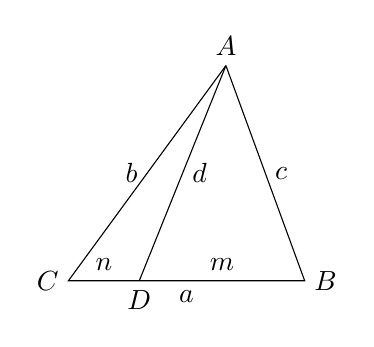
\begin{tikzpicture}
    % titik-titik segitiga
    \coordinate[label=left:$C$]  (C) at (-1.5cm,-1.cm);
    \coordinate[label=right:$B$] (B) at (1.5cm,-1.0cm);
    \coordinate[label=above:$A$] (A) at (0.5cm,1.732cm);
    % titik-titik cevian
    \coordinate[label=below:$D$] (D) at ($(C)!0.3!(B)$);
    
    % pembuatan segitiga
    \draw (A) -- node[right]{$c$} (B) -- node[above]{$m$} (D) -- node[above]{$n$} (C) -- node[left]{$b$} (A);
    
    
    % pembuatan cevian
    \draw (B) --node[below]{$a$}(C);
    \draw (A) --node[right]{$d$}(D);
    \end{tikzpicture}
\end{center}
\subsection{Latihan Soal Dalil Stewart}
\begin{enumerate}
    \item (OSK 2016) Pada segitiga $ABC$, titik $M$ terletak pada $BC$ sehingga $AB=7, AM=3, BM=5$, dan $MC=6$. Panjang $AC$ adalah \dots

    \item (HMMT 1999) Dalam segitiga $ABD$, $F$ berada pada segmen $AD$, $E$ berada pada sinar $BF$, $G$ berada pada segmen $BD$, dan $C$ adalah titik perpotongan dari $FG$ dan $ED$. Diketahui bahwa $AB = 15$, $BD = 18$, $AF = 15$, $DF = 12$, $BE = 24$, dan $CF = 17$. Temukan rasio $BG : FG$.
    % https://drive.google.com/drive/search?q=parent:0B-4OltLGFEDFeG92VENBbmdZODA%20type:pdf%20menelaus
\end{enumerate}
\subsection{Dalil Ceva}
Jika pada segitiga $ABC$, titik $D,E,F$ berturut-turut berada di segmen $BC$,$CA$,$AB$, maka 
$AD,BE,CF$ konkuren atau berpotongan di satu titik jika dan hanya jika $$\dfrac{AF}{FB} \cdot \dfrac{BD}{DC} \cdot \dfrac{CE}{EA} = 1.$$
\begin{center}
    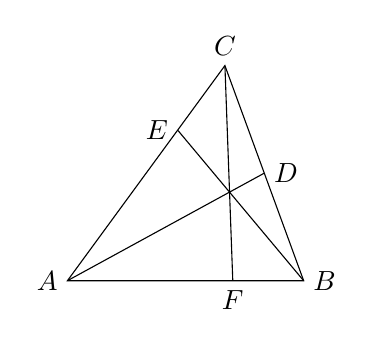
\begin{tikzpicture}
    % titik-titik segitiga
    \coordinate[label=left:$A$]  (A) at (-1.5cm,-1.cm);
    \coordinate[label=right:$B$] (B) at (1.5cm,-1.0cm);
    \coordinate[label=above:$C$] (C) at (0.5cm,1.732cm);
    
    % pembuatan segitiga
    \draw (A) -- (B) -- (C) -- cycle;
    
    % titik-titik cevian
    \coordinate[label=below:$F$] (F) at ($(A)!0.7!(B)$);
    \coordinate[label=right:$D$] (D) at ($(B)!0.5!(C)$);
    \coordinate[label=left:$E$]  (E) at ($(C)!0.3!(A)$);
    
    % pembuatan cevian
    \draw (A) -- (D);
    \draw (B) -- (E);
    \draw (C) -- (F);
    \end{tikzpicture}
\end{center}
\subsection{Latihan Soal Dalil Ceva}
\begin{enumerate}
    \item (OSK 2015) Pada segitiga $ABC$, garis tinggi $AD$, garis bagi $BE$ dan garis berat $CF$ berpotongan di satu titik. Jika panjang $AB = 4$ dan $BC = 5$, dan $CD = \frac{m^2}{n^2}$ dengan $m$ dan $n$ relatif prima, maka nilai dari $m - n$ adalah \ldots
\end{enumerate}

\subsection{Dalil Menelaus}
Jika pada segitiga $ABC$, titik $P,Q,R$ berturut-turut berada pada garis (bisa di perpanjangan segmen) $BC$,$CA$, $AB$, maka $P,Q,R$ segaris jika dan hanya jika
$$\dfrac{AR}{RB} \cdot \dfrac{BP}{PC} \cdot \dfrac{CQ}{QA} = 1.$$
\begin{center}
    \begin{asy}
        unitsize(10);
        defaultpen(fontsize(8));
        pair P=(7,6), Q=(0,0), C=(10,0), A=(4,0), B=(6,8), R;
        draw((A)--(B)--(C)--cycle,blue+0.75);
        draw(P--R--Q--A);
        R=intersectionpoint(A--B,Q--P);
        dot(A^^B^^C^^P^^Q^^R);
        label("A",A,(0,-1));label("B",B,(1,0));label("C",C,(1,0));label("P",P,(1,1));label("Q",Q,(-1,0));label("R",R,(-1,1));
    \end{asy}
\end{center}
\subsection{Latihan Soal Dalil Menelaus}
\begin{enumerate}
    \item Dalam segitiga $ABD$, $F$ berada pada segmen $AD$, $E$ berada pada sinar $BF$, $G$ berada pada segmen $BD$, dan $C$ adalah titik perpotongan dari $FG$ dan $ED$. Diketahui bahwa $AB = 15$, $BD = 18$, $AF = 15$, $DF = 12$, $BE = 24$, dan $CF = 17$. Temukan rasio $BG : FG$.
    % https://drive.google.com/drive/search?q=parent:0B-4OltLGFEDFeG92VENBbmdZODA%20type:pdf%20menelaus

    \item (OSK 2022) Diberikan $ABC$ siku-siku sama kaki dengan $BC=AB$. Misalkan $L$ titik tengah $BC$ dan $P$ pada sisi $AC$ sehingga $BP \perp AL$. Jika $CP=30\sqrt{2}$, maka panjang $AB$ adalah \ldots

    \item Diberikan segitiga $ABC$ dengan panjang $BC = 36$. Misalkan $D$ adalah titik tengah $BC$ dan $E$ adalah titik tengah $AD$. Misalkan pula bahwa $F$ adalah perpotongan $BE$ dengan $AC$. Jika diketahui bahwa $AB$ menyinggung lingkaran luar segitiga $BFC$, hitunglah panjang $BF$.
\end{enumerate}
\subsection{Dalil Ptolemy}
    Diketahui sebuah segiempat siklis $ABCD$ maka berlaku
    $$AB \cdot CD + BC \cdot DA = AC \cdot BD.$$

\begin{center}
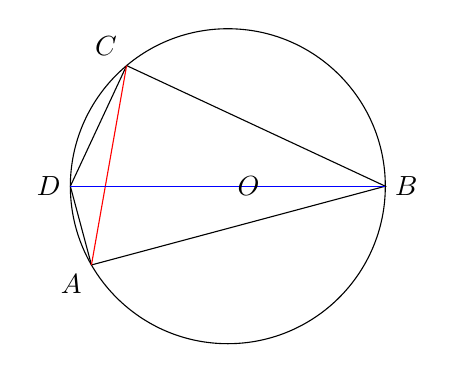
\begin{tikzpicture}
\coordinate (O) at (0,0);
\coordinate (B) at (0:2cm);
\coordinate (A) at (210:2cm);
\coordinate (D) at (180:2cm);
\coordinate (C) at (130:2cm);

\draw (O) circle (2cm);

\draw (A) -- (B) -- (C) -- (D) -- cycle;
\draw[red] (A) -- (C);
\draw[blue] (B) -- (D);

\node[right] at (B) {$B$};
\node[below left] at (A) {$A$};
\node[left] at (D) {$D$};
\node[above left] at (C) {$C$};
\node[right] at (O) {$O$};
\end{tikzpicture}
\end{center}
\subsection{Latihan Soal Dalil Ptolemy}
\begin{enumerate}
    \item Diberikan sebuah segiempat siklis $ABCD$ dengan $ABC$ adalah segitiga sama sisi. Jika $AD=2$ dan $CD=3$, panjang $BD=\dots$
\end{enumerate}	
\end{document}
